% opsph.tex
% opérateurs sphériques sur la sphère

\chapter{Approximation des opérateurs sphériques sur la Cubed-sphere}

La résolution des équations de type Shallow-Water \REF la sphère $\mathbb{S}_a^2$ demande le calcul approché d'opérateurs classiques. Les opérateurs différentiels sont indispensables pour la discrétisation spatiale. On pense en particulier aux opérateurs divergence, gradient ou rotationnel. Dans cette section, nous les définissons sur la Cubed-sphere. 
Nous avons vu dans le cas 1D qu'un opérateur de filtrage peut être utile pour supprimer les modes de type "$+1/-1$" qui perturbent le calcul lors de la discrétisation en temps. Nous définissons les opérateurs de filtrages permettant d'aboutir au filtrage qui sera utilisé dans la discrétisation temporelle des équations.
Dans ce chapitre, les notations employées telles que $\xi$, $\eta$, $\alpha$, ... sont celles employées dans le chapitre \REF concernant la Cubed-sphere.

\section{Opérateurs différentiels sur la Cubed-sphere}

\subsection{Définition des opérateurs}
Soit $\mathbf{x}_{i,j}^k$ un point de la Cubed-sphere avec $- N/2 \leq i,j \leq N/2$ et $k = (I) \cdots (VI)$. Alors il existe deux grands cercles $C_i^{(1)}$ et $C_j^{(2)}$ tels que $\mathbf{x}_{i,j}^k \in C_i^{(1)} \cap C^{(2)}_j$. $\alpha$ et $\beta$ sont respectivement les angles paramétrant $C_i^{(1)}$ et $C_j^{(2)}$.

On a définit le gradient en $\mathbf{x}_{i,j}^k$ par 
\begin{equation}
\nabla_T h = \dfrac{\partial h}{\partial \alpha}_{|C^{(2)}_j} \mathbf{g}^{\alpha} + \dfrac{\partial h}{\partial \beta}_{|C^{(1)}_i} \mathbf{g}^{\beta},
\end{equation}
où $h : \mathbf{x} \in \mathbb{S}_a^2 \mapsto h(\mathbf{x})$ est une fonction régulière sur la sphère.

Le cercle $C_i^{(1)}$ (resp. $C_j^{(2)}$) est une isocline $\xi = \xi_i$ (resp $\eta = \eta_j$) constant. D'après le théorème \eqref{th:gradient_xieta}, le gradient est 
\begin{equation}
\nabla_T h = \dfrac{\partial h}{\partial \xi}_{|\eta_j} \mathbf{g}^{\xi} + \dfrac{\partial h}{\partial \eta}_{|\xi_i} \mathbf{g}^{\eta}.
\end{equation}
On remarque que si l'on est capable de calculer les dérivées partielles $\partial_{\xi}$ et $\partial_{\eta}$ le long des grands cercles, alors on est capable de déterminer la valeur du gradient.

Soit $\mathbf{v} : \mathbf{x} \in \mathbb{S}_a^2 \mapsto \mathbf{v}(\mathbf{x}) \in \mathbb{T}_{\mathbf{x}} \mathbb{S}_a^2$ un champ de vecteur tangent à la sphère. On définit la \textit{divergence} et le \textit{rotationnel} de $\mathbf{v}$ notés $\nabla_T \cdot \mathbf{v}$ et $\nabla_T \wedge \mathbf{v}$.

\begin{definition}
Soit $\mathbf{v} : \mathbf{x} \in \mathbb{S}_a^2 \mapsto \mathbf{v}(\mathbf{x}) \in \mathbb{T}_{\mathbf{x}} \mathbb{S}_a^2$ un champ de vecteur régulier sur la sphère. Alors la divergence de $\mathbf{v}$ en $\mathbf{x} \in C_i^{(1)} \cap C_j^{(2)}$ est donnée par
\begin{equation}
\nabla_T \cdot \mathbf{v} = \dfrac{\partial \mathbf{v}}{\partial \alpha}_{|C^{(2)}_j} \cdot \mathbf{g}^{\alpha} + \dfrac{\partial \mathbf{v}}{\partial \beta}_{|C^{(1)}_i} \cdot \mathbf{g}^{\beta}.
\end{equation}
\label{def:divergence}
La notation $\cdot$ désigne le produit scalaire usuel dans $\mathbb{R}^3$.
\end{definition}
Le rotationnel d'un champ de vecteurs représente la tendance des lignes de courant de $\mathbf{v}$ à tourner autour d'un point. Il est définit par

\begin{definition}
Soit $\mathbf{v} : \mathbf{x} \in \mathbb{S}_a^2 \mapsto \mathbf{v}(\mathbf{x}) \in \mathbb{T}_{\mathbf{x}} \mathbb{S}_a^2$ un champ de vecteur régulier sur la sphère. Alors le rotationnel de $\mathbf{v}$ en $\mathbf{x} \in C_i^{(1)} \cap C_j^{(2)}$ est donnée par
\begin{equation}
\nabla_T \wedge \mathbf{v} =  \mathbf{g}^{\alpha} \wedge \dfrac{\partial \mathbf{v}}{\partial \alpha}_{|C^{(2)}_j} + \mathbf{g}^{\beta} \wedge \dfrac{\partial \mathbf{v}}{\partial \beta}_{|C^{(1)}_i}
\end{equation}
où $\wedge$ désigne le produit vectoriel.
\label{def:rotationnel}
\end{definition}
La \textit{vorticité} du champ de vecteurs $\mathbf{v}$ est la composante normale du rotationnel :
\begin{equation}
\vort ( \mathbf{v} ) = \left( \nabla_T \wedge \mathbf{v} \right) \cdot \mathbf{n}
\label{eq:vorticité}
\end{equation}
avec $\mathbf{n}$ le vecteur unitaire extérieur à la sphère en $\mathbf{x} \in \mathbb{S}_a^2$, vérifiant l'égalité
\begin{equation}
\mathbf{n} = \dfrac{1}{a} \mathbf{x}.
\end{equation}

En utilisant la proposition \ref{prop: g_alpha g_beta fct de g_xi g_eta}, il est facile de montrer que des égalités permettant de calculer les opérateurs à l'aide des dérivées en $\xi$ et en $\eta$.

\begin{theoreme}
Soit $h : \mathbf{x} \in \mathbb{S}_a^2 \mapsto h(\mathbf{x})$ une fonction régulière et $\mathbf{v} : \mathbf{x} \in \mathbb{S}_a^2 \mapsto \mathbf{v}(\mathbf{x}) \in \mathbb{T}_{\mathbf{x}} \mathbb{S}_a^2$ un champ de vecteurs régulier. Alors en $\mathbf{x}_{i,j}^k$ un point de la Cubed-Sphere, les égalités suivantes sont satisfaites :
\begin{itemize}
\item \textbf{Gradient} :
\begin{equation}
\nabla_T h = \dfrac{\partial h}{\partial \xi}_{|\eta_j} \mathbf{g}^{\xi} + \dfrac{\partial h}{\partial \eta}_{|\xi_i} \mathbf{g}^{\eta},
\end{equation}

\item \textbf{Divergence} :
\begin{equation}
\nabla_T \cdot \mathbf{v} = \dfrac{\partial \mathbf{v}}{\partial \xi}_{|\eta_j} \cdot \mathbf{g}^{\xi} + \dfrac{\partial \mathbf{v}}{\partial \eta}_{|\xi_i} \cdot \mathbf{g}^{\eta},
\label{eq:divergence_v1}
\end{equation}

\item \textbf{Vorticité} :
\begin{equation}
\vort( \mathbf{v} ) = \left( \nabla_T \cdot \mathbf{v} \right) \cdot \mathbf{n} =  \left( \mathbf{g}^{\xi} \wedge \dfrac{\partial \mathbf{v}}{\partial \xi}_{|\eta_j} + \mathbf{g}^{\eta} \wedge \dfrac{\partial \mathbf{v}}{\partial \eta}_{|\xi_i} \right) \cdot \mathbf{n}.
\end{equation}
\end{itemize} 
\end{theoreme}

Pour calculer une valeur approchée des opérateurs gradient, divergence et rotationnel aux points du maillage de la Cubed-Sphere, il faut calculer une valeur approchée de la dérivée d'une fonction le long d'un grand cercle. C'est à dire, calculer $f_{\xi,i,j}$ et $f_{\eta,i,j}$ tels que 
\begin{equation}
\left\lbrace
\begin{array}{rl}
f_{\xi,i,j} \rightarrow \partial_{\xi} f ( \mathbf{x}_{i,j}^k) & \text{ lorsque } \Delta \xi \rightarrow 0\\
f_{\eta,i,j} \rightarrow \partial_{\eta} f ( \mathbf{x}_{i,j}^k) & \text{ lorsque } \Delta \eta \rightarrow 0
\end{array}
\right.
\end{equation}
La section suivante consiste à détailler une procédure pour calculer ces dérivées partielles approchées et à déterminer l'erreur de troncature effectuée lors du calcul.





\subsection{Approximation de dérivées sur les grands cercles}

On pose $f : \mathbf{x}\in \mathbb{S}_a^2 \mapsto f(\mathbf{x})$ la fonction que l'on souhaite dérivée le long des grands cercles aux points du maillage de la Cubed-Sphere.
Si $\mathbf{x}_{i,j}^k$ est un point de la Cubed-Sphere avec $k = (I) \cdots (VI)$, ainsi que $-N/2 \leq i,j \leq N/2$. On souhaite calculer une valeur approchée de 
$
\partial_{\xi} f (\mathbf{x}_{i,j}^k)$ et $\partial_{\eta} f (\mathbf{x}_{i,j}^k)$.
On suppose $k = (I)$, la méthode est la même sur les autres panels. Il existe deux grands cercles de la Cubed-Sphere $C_i^{(1)}$ et $C_j^{(2)}$ tels que 
\begin{equation}
\mathbf{x}_{i,j}^k \in C_i^{(1)} \cap C^{(2)}_j.
\end{equation}
$C^{(1)}_i$ est une isoligne en $\xi = \xi_i$ constant et $C^{(2)}_j$ est une isoligne en $\eta = \eta_j$ constant.
Pour calculer une valeur approchée de $\partial_{\xi} f (\mathbf{x}_{i,j}^{(I)})$, on souhaite connaître toutes les valeurs de $f$ aux points équirépartis le long du cercle $C^{(2)}_j$. On pose $\mathbf{m}_p$ avec $0 \leq p \leq 4N-1$ les points de $C^{(2)}_j$ construits de la manière suivante :
\begin{itemize}
\item si $0 \leq p \leq N$ alors $\mathbf{m}_p = \mathbf{x}^{(I)}_{p-N/2,j}$, il s'agit des points du cercle $C^{(2)}_j$ associés au panel $(I)$ sur le maillage. Ils sont représentés par des ronds bleus sur les figures \ref{fig:patron_cs} et \ref{fig: panel II_interp},
\item si $N+1 \leq p \leq 2N-1$ alors les points ne font pas partis du maillages. Il s'agit des points d'intersections de $C^{(2)}_j$ avec les isoligne $\xi = \xi_i^{(II)}$ du panel $(II)$. C'est à dire l'intersection de $C^{(2)}_j$ avec les cercles de $(II_{\beta})$. Ces points sont représentés par les carrés bleus dans les figures \ref{fig:patron_cs} et \ref{fig: panel II_interp}. Les coordonnées de ces points ont été calculées dans la partie \REF.
\item si $2N \leq p \leq 3N$ alors $\mathbf{m}_p = \mathbf{x}^{(III)}_{p-3N/2}$. Il s'agit des points de la Cubed-Sphere du panel $(III)$ représentés par des ronds bleus sur la figure \ref{fig:patron_cs},
\item si $3N+1 \leq p \leq 4N-1$ alors $\mathbf{m}_p$ est constitués des points d'intersections de $C^{(2)}_j$ avec les cercles de $(IV_{\beta})$. Il ne s'agit pas de points de la grille. Ces points sont représentés par les carrés bleus dans la figure \ref{fig:patron_cs}.
\end{itemize}

\begin{figure}
\begin{center}
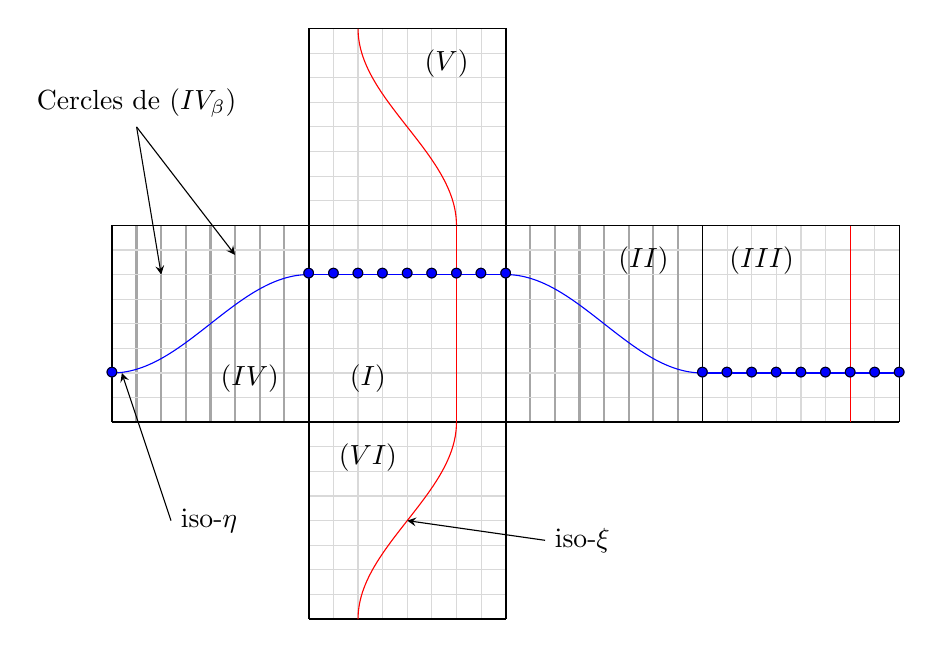
\begin{tikzpicture}[scale=2.5]
	\foreach \x in {1,...,7}
		{ \draw [color=gray!70, line width=0.8pt] (0.125*\x,1) -- (0.125*\x,2) ;
		\draw [color=gray!30] (0,1+0.125*\x) -- (1,1+0.125*\x) ;
		\draw [color=gray!30] (1+0.125*\x,1) -- (1+0.125*\x,2) ;
		\draw [color=gray!30] (1,1+0.125*\x) -- (2,1+0.125*\x) ;
		\draw [color=gray!70, line width=0.8pt] (2+0.125*\x,1) -- (2+0.125*\x,2) ;
		\draw [color=gray!30] (2,1+0.125*\x) -- (3,1+0.125*\x) ;
		\draw [color=gray!30] (3+0.125*\x,1) -- (3+0.125*\x,2) ;
		\draw [color=gray!30] (3,1+0.125*\x) -- (4,1+0.125*\x) ;
		\draw [color=gray!30] (1+0.125*\x,0) -- (1+0.125*\x,1) ;
		\draw [color=gray!30] (1,0.125*\x) -- (2,0.125*\x) ;
		\draw [color=gray!30] (1+0.125*\x,2) -- (1+0.125*\x,3) ;		
		\draw [color=gray!30] (1,2+0.125*\x) -- (2,2+0.125*\x) ;
		}
	

	\draw [line width=0.6pt] (1,3) -- (2,3) ; 
	\draw [line width=0.6pt] (0,2) -- (4,2) ; 	
	\draw [line width=0.6pt] (0,1) -- (4,1) ; 
	\draw [line width=0.6pt] (1,0) -- (2,0) ; 
	
	\draw [line width=0.6pt] (0,2) -- (0,1) ;
	\draw [line width=0.6pt] (1,3) -- (1,0) ;
	\draw [line width=0.6pt] (2,3) -- (2,0) ;
	\draw [line width=0.6pt] (3,2) -- (3,1) ;
	\draw [line width=0.6pt] (4,2) -- (4,1) ; 
	
	\draw (0.7,1.1) node[above]{$(IV)$} ; 
	\draw (1.3,1.1) node[above]{$(I)$} ; 
	\draw (2.7,1.7) node[above]{$(II)$} ;
	\draw (3.3,1.7) node[above]{$(III)$} ;  
	\draw (1.7,2.7) node[above]{$(V)$} ;  
	\draw (1.3,0.7) node[above]{$(VI)$} ; 
	
	\draw [samples=100,domain=0:1,color=blue] plot({\x},{1.5-(2*0.125)*cos(180*\x)});
	\draw [samples=100,domain=1:2,color=blue] plot({\x},{1.5+2*0.125});
	\draw [samples=100,domain=1:2,color=blue] plot({\x+1},{1.5-2*0.125*cos(180*\x)});
	\draw [samples=100,domain=3:4,color=blue] plot({\x},{1.5-2*0.125});
	\draw [>=stealth, <-] (0.05,1.25) -- (0.3,0.5) ;
	\draw  (0.3,0.5) node[right] {iso-$\eta$} ;
	
	\draw [samples=100,domain=0:1,color=red] plot({1.5-2*0.125*cos(180*\x)},{\x});
	\draw [samples=100,domain=1:2,color=red] plot({1.5+2*0.125},{\x});
	\draw [samples=100,domain=1:2,color=red] plot({1.5-2*0.125*cos(180*\x)},{\x+1});
	\draw [samples=100,domain=1:2,color=red] plot({4-2*0.125},{\x});
	\draw [>=stealth, <-] (1.5,0.5) -- (2.2,0.4) ;
	\draw  (2.2,0.4) node[right] {iso-$\xi$} ;
	
	\draw  (0,1+2*0.125) node[color=blue] {$\bullet$} ;
	\draw (0,1+2*0.125) node {$\circ$} ;
	
	\foreach \k in {0,...,8}
		{\draw  (1+0.125*\k,1.5+2*0.125) node[color=blue] {$\bullet$} ;
	   	\draw (1+0.125*\k,1.5+2*0.125) node {$\circ$} ;
	   	\draw  (3+0.125*\k,1+2*0.125) node[color=blue] {$\bullet$} ;
	   	\draw (3+0.125*\k,1+2*0.125) node {$\circ$} ;
	   	}
	   	
	\foreach \x in {1,...,7}
		{\draw  ({0.125*\x},{1.5-2*0.125*cos(180*0.125*\x)}) node[color=blue] {\begin{tiny}$\blacksquare$\end{tiny}} ;
	   	\draw ({0.125*\x},{1.5-2*0.125*cos(180*0.125*\x)}) node {\begin{tiny}$\square$\end{tiny}} ;
	   	\draw  ({2+0.125*\x},{1.5-2*0.125*cos(180*0.125*\x+180)}) node[color=blue] {\begin{tiny}$\blacksquare$\end{tiny}} ;
	   	\draw  ({2+0.125*\x},{1.5-2*0.125*cos(180*0.125*\x+180)}) node {\begin{tiny}$\square$\end{tiny}} ;
	   	}
	   	
	\draw [>=stealth, <-] (0.25,1.75) -- (0.125,2.5) ;
	\draw [>=stealth, <-] (0.625,1.85) -- (0.125,2.5) ;
	\draw  (0.125,2.5) node[above] {Cercles de $(IV_{\beta})$} ;
\end{tikzpicture}
\caption{Les grands cercles associés aux panels $(I)$ et $(III)$ ne sont pas passent pas par des points du la Cubed-Sphere sur les panels $(II)$ et $(IV)$.}
\label{fig:patron_cs}
\end{center}
\end{figure}




\begin{figure}[htbp]
\begin{center}
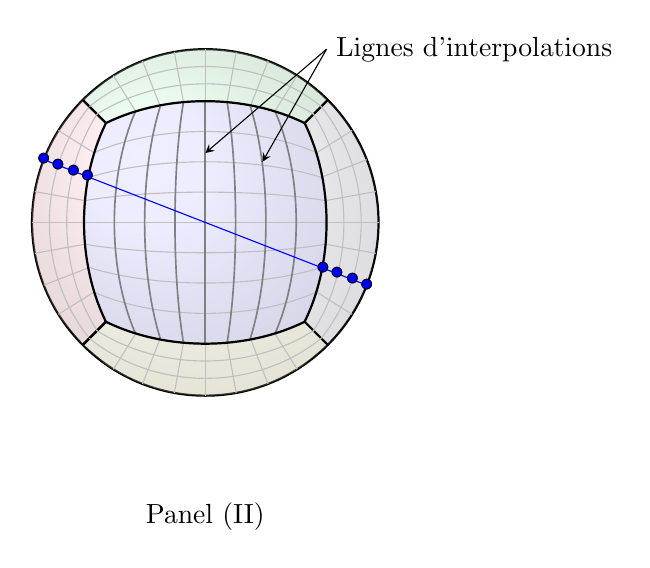
\begin{tikzpicture}[scale=2.2]
	\draw [line width=0.8pt] (0,0) circle (1cm);
    \shade[ball color=blue!10!white,opacity=0.20] (0,0) circle (1cm);	
	
	\filldraw[draw=black,fill=blue!30!white,opacity=0.20]
	plot [smooth,domain=-35:35] ({0.7*cos(\x)},{sin(\x)})
	-- plot [smooth,domain=55:125] ({cos(\x)},{0.7*sin(\x)})
	-- plot [smooth,domain=150:215] ({0.7*cos(\x)},{sin(\x)})
	-- plot [smooth,domain=240:300] ({cos(\x)},{0.7*sin(\x)})
	-- cycle;	
	\draw [samples=100,domain=48:132, color=gray!50] plot({cos(\x)},{0.35*sin(\x)});
	\draw [samples=100,domain=48:132, color=gray!50] plot({cos(\x)},{-.35*sin(\x)});
	\draw [samples=100,domain=46:134, color=gray!50] plot({cos(\x)},{0.175*sin(\x)});
	\draw [samples=100,domain=46:134, color=gray!50] plot({cos(\x)},{-.175*sin(\x)});
	\draw [samples=100,domain=50:130, color=gray!50] plot({cos(\x)},{0.525*sin(\x)});
	\draw [samples=100,domain=50:130, color=gray!50] plot({cos(\x)},{-.525*sin(\x)});
	\draw [samples=100,domain=45:135, color=gray!50] plot({cos(\x)},{0*sin(\x)});

	\draw [rotate=90, samples=100,domain=48:132, color=gray, line width=0.6pt] plot({cos(\x)},{0.35*sin(\x)});
	\draw [rotate=90, samples=100,domain=48:132, color=gray, line width=0.6pt] plot({cos(\x)},{-.35*sin(\x)});
	\draw [rotate=90, samples=100,domain=46:134, color=gray, line width=0.6pt] plot({cos(\x)},{0.175*sin(\x)});
	\draw [rotate=90, samples=100,domain=46:134, color=gray, line width=0.6pt] plot({cos(\x)},{-.175*sin(\x)});
	\draw [rotate=90, samples=100,domain=50:130, color=gray, line width=0.6pt] plot({cos(\x)},{0.525*sin(\x)});
	\draw [rotate=90, samples=100,domain=50:130, color=gray, line width=0.6pt] plot({cos(\x)},{-.525*sin(\x)});
	\draw [rotate=90, samples=100,domain=45:135, color=gray, line width=0.6pt] plot({cos(\x)},{0*sin(\x)});

	\filldraw[draw=black,fill=red!30!white,opacity=0.20]
	plot [smooth,domain=145:215] ({.7*cos(\x)},{sin(\x)})
	-- plot [smooth] (-.573,-.573) -- (-.707,-.707)
	-- plot [smooth,domain=215:145] ({cos(\x)},{sin(\x)})
	-- plot [smooth] (-.707,.707) -- (-.573,.573)
	-- cycle;	
	\draw [line width=0.8pt] (-.573,-.573) -- (-.707,-.707) ;
	\draw [line width=0.8pt] (-.573,.573) -- (-.707,.707) ;
	\draw [color=gray!50] (-.669,.260) -- (-.9321,.3622) ;
	\draw [color=gray!50] (-.669,-.260) -- (-.9321,-.3622) ;
	\draw [color=gray!50] (-.6946,.1259) -- (-.9840,.1783) ;
	\draw [color=gray!50] (-.6946,-.1259) -- (-.9840,-.1783) ;
	\draw [color=gray!50] (-.6427,.4022) -- (-.8477,.5305) ;
	\draw [color=gray!50] (-.6427,-.4022) -- (-.8477,-.5305) ;
	\draw [color=gray!50] (-.707,0) -- (-1,0) ;
	\draw [samples=100,domain=141:219, color=gray!50] plot({0.8*cos(\x)},{sin(\x)});
	\draw [samples=100,domain=138:222, color=gray!50] plot({0.9*cos(\x)},{sin(\x)});
	
	\filldraw[draw=black,fill=green!30!white,opacity=0.20]
	plot [smooth,domain=55:125] ({cos(\x)},{0.7*sin(\x)})
	-- plot [smooth] (-.573,.573) -- (-.707,.707)
	-- plot [smooth,domain=125:55] ({cos(\x)},{sin(\x)})
	-- plot [smooth] (.707,.707) -- (.573,.573)
	-- cycle;	
	\draw [line width=0.8pt] (-.573,.573) -- (-.707,.707) ;
	\draw [line width=0.8pt] (.707,.707) -- (.573,.573) ;
	\draw [rotate=-90,color=gray!50] (-.669,.260) -- (-.9321,.3622) ;
	\draw [rotate=-90,color=gray!50] (-.669,-.260) -- (-.9321,-.3622) ;
	\draw [rotate=-90,color=gray!50] (-.6946,.1259) -- (-.9840,.1783) ;
	\draw [rotate=-90,color=gray!50] (-.6946,-.1259) -- (-.9840,-.1783) ;
	\draw [rotate=-90,color=gray!50] (-.6427,.4022) -- (-.8477,.5305) ;
	\draw [rotate=-90,color=gray!50] (-.6427,-.4022) -- (-.8477,-.5305) ;
	\draw [rotate=-90,color=gray!50] (-.707,0) -- (-1,0) ;
	\draw [rotate=-90,samples=100,domain=141:219, color=gray!50] plot({0.8*cos(\x)},{sin(\x)});
	\draw [rotate=-90,samples=100,domain=138:222, color=gray!50] plot({0.9*cos(\x)},{sin(\x)});
	
	\filldraw[draw=black,fill=yellow!30!white,opacity=0.20]
	plot [smooth,domain=55:125] ({cos(\x)},{-.7*sin(\x)})
	-- plot [smooth] (-.573,-.573) -- (-.707,-.707)
	-- plot [smooth,domain=125:55] ({cos(\x)},{-sin(\x)})
	-- plot [smooth] (.707,-.707) -- (.573,-.573)
	-- cycle;	
	\draw [line width=0.8pt] (-.573,-.573) -- (-.707,-.707) ;
	\draw [line width=0.8pt] (.707,-.707) -- (.573,-.573) ;
	\draw [rotate=90,color=gray!50] (-.669,.260) -- (-.9321,.3622) ;
	\draw [rotate=90,color=gray!50] (-.669,-.260) -- (-.9321,-.3622) ;
	\draw [rotate=90,color=gray!50] (-.6946,.1259) -- (-.9840,.1783) ;
	\draw [rotate=90,color=gray!50] (-.6946,-.1259) -- (-.9840,-.1783) ;
	\draw [rotate=90,color=gray!50] (-.6427,.4022) -- (-.8477,.5305) ;
	\draw [rotate=90,color=gray!50] (-.6427,-.4022) -- (-.8477,-.5305) ;
	\draw [rotate=90,color=gray!50] (-.707,0) -- (-1,0) ;
	\draw [rotate=90,samples=100,domain=141:219, color=gray!50] plot({0.8*cos(\x)},{sin(\x)});
	\draw [rotate=90,samples=100,domain=138:222, color=gray!50] plot({0.9*cos(\x)},{sin(\x)});
	
	\draw [rotate=180,color=gray!50] (-.669,.260) -- (-.9321,.3622) ;
	\draw [rotate=180,color=gray!50] (-.669,-.260) -- (-.9321,-.3622) ;
	\draw [rotate=180,color=gray!50] (-.6946,.1259) -- (-.9840,.1783) ;
	\draw [rotate=180,color=gray!50] (-.6946,-.1259) -- (-.9840,-.1783) ;
	\draw [rotate=180,color=gray!50] (-.6427,.4022) -- (-.8477,.5305) ;
	\draw [rotate=180,color=gray!50] (-.6427,-.4022) -- (-.8477,-.5305) ;
	\draw [rotate=180,color=gray!50] (-.707,0) -- (-1,0) ;
	\draw [rotate=180,samples=100,domain=141:219, color=gray!50] plot({0.8*cos(\x)},{sin(\x)});
	\draw [rotate=180,samples=100,domain=138:222, color=gray!50] plot({0.9*cos(\x)},{sin(\x)});
	
	\draw [samples=100,domain=55:125, line width=0.8pt] plot({cos(\x)},{0.7*sin(\x)});
	\draw [samples=100,domain=55:125, line width=0.8pt] plot({cos(\x)},{-.7*sin(\x)});
	\draw [samples=100,domain=145:215, line width=0.8pt] plot({.7*cos(\x)},{sin(\x)}); 
	\draw [samples=100,domain=145:215, line width=0.8pt] plot({-.7*cos(\x)},{sin(\x)}); 
	
	\draw [color=blue] (-.9321,.3622) -- (.9321,-.3622) ;
	\draw  (-.9321,.3622) node[color=blue] {$\bullet$} ;
	\draw (-.9321,.3622) node {$\circ$} ;	
	\draw  (.9321,-.3622) node[color=blue] {$\bullet$} ;
	\draw (.9321,-.3622) node {$\circ$} ;
	\draw  (-.85,0.3886*.85) node[color=blue] {$\bullet$} ;
	\draw (-.85,0.3886*.85) node {$\circ$} ;	
	\draw (.85,-0.3886*.85) node[color=blue] {$\bullet$} ;
	\draw (.85,-0.3886*.85) node {$\circ$} ;	
	\draw  (-.76,0.3886*.76) node[color=blue] {$\bullet$} ;
	\draw (-.76,0.3886*.76) node {$\circ$} ;	
	\draw (.76,-0.3886*.76) node[color=blue] {$\bullet$} ;
	\draw (.76,-0.3886*.76) node {$\circ$} ;
	\draw  (-.68,0.3886*.68) node[color=blue] {$\bullet$} ;
	\draw (-.68,0.3886*.68) node {$\circ$} ;	
	\draw (.68,-0.3886*.68) node[color=blue] {$\bullet$} ;
	\draw (.68,-0.3886*.68) node {$\circ$} ;	
	\draw (-.52,0.3886*.52) node[color=blue] {\begin{tiny}$\blacksquare$ \end{tiny}} ;
	\draw (-.52,0.3886*.52) node {\begin{tiny}$\square$ \end{tiny}} ;
	\draw (.52,-0.3886*.52) node[color=blue] {\begin{tiny}$\blacksquare$ \end{tiny}} ;
	\draw (.52,-0.3886*.52) node {\begin{tiny}$\square$ \end{tiny}} ;
	\draw (-.36,0.3886*.36) node[color=blue] {\begin{tiny}$\blacksquare$ \end{tiny}} ;
	\draw (-.36,0.3886*.36) node {\begin{tiny}$\square$ \end{tiny}} ;
	\draw (.36,-0.3886*.36) node[color=blue] {\begin{tiny}$\blacksquare$ \end{tiny}} ;
	\draw (.36,-0.3886*.36) node {\begin{tiny}$\square$ \end{tiny}} ;
	\draw (-.18,0.3886*.18) node[color=blue] {\begin{tiny}$\blacksquare$ \end{tiny}} ;
	\draw (-.18,0.3886*.18) node {\begin{tiny}$\square$ \end{tiny}} ;
	\draw (.18,-0.3886*.18) node[color=blue] {\begin{tiny}$\blacksquare$ \end{tiny}} ;
	\draw (.18,-0.3886*.18) node {\begin{tiny}$\square$ \end{tiny}} ;
	\draw (0,0) node[color=blue] {\begin{tiny}$\blacksquare$ \end{tiny}} ;
	\draw (0,0) node {\begin{tiny}$\square$ \end{tiny}} ;
	
	\draw [>=stealth, <-] (.33,.35) -- (.7,1) ;
	\draw [>=stealth, <-] (0,.4) -- (.7,1) ;
	\draw  (0.7,1) node[right] {Lignes d'interpolations} ;
	
	\draw  (0,-1.7) node {Panel (II)} ;

\end{tikzpicture}
\end{center}
\caption{La ligne bleue représente une isoligne $\eta=\eta_j$ du panel $(I)$ vue depuis le panel $(II)$. les cercles bleus représentent des points de la Cubed-Sphere contenues dans l'isoligne $\eta=\eta_j$, les carrés bleus sont des points de l'isoligne $\eta=\eta_j$ qui ne sont pas sur la Cubed-Sphere.}
\label{fig: panel II_interp}
\end{figure}  

La périodicité sur les grands cercles permet d'assurer que $\mathbf{m}_p = \mathbf{m}_{p+4N}$ pour tout $p \in \mathbb{Z}$. De plus, la construction de la Cubed-Sphere, permet d'assurer un paramétrage du grand cercle $C^{(2)}_j$. Chaque point est associé à des coordonnées $(\xi_p, \eta_p)$. Les valeurs de $\xi_p$ donnent un paramétrage des points $\mathbf{m}_p$ le long du grand cercle. On a de plus
\begin{equation}
\xi_{p+1} = \xi_p + \Delta \xi
\end{equation}
Si $f_p = f(\mathbf{m}_p)$ est connue pour tout $p$ vérifiant $0 \leq p \leq 4N-1$ alors on peut calculer la dérivée approchée $f_{\xi,i,j}^k$ de $\partial_{\xi}f(\mathbf{x}_{i,j}^k)$ à l'ordre $4$ grâce à la formule de dérivation hermitienne \eqref{eq:comp4}
\begin{equation}
f_{\xi,i,j}^k = \delta_{4,\xi}^H f_p.
\end{equation}
Cependant, les valeurs de $f_p$ ne sont pas toutes connues car les points $\mathbf{m}_p$ ne sont pas des points du maillages lorsque $N+1 \leq p \leq 2N-1$ ou $3N+4 \leq p \leq 4N-1$. Il faut donc construire un procéder permettant d'obtenir des valeurs en ces points. Le procédé utilisé dans ce travail est basé sur une interpolation à l'aide de Splines Cubiques.

On souhaite calculer une valeur $f_p$ approchant $f(\mathbf{m}_p)$ avec $N+1 \leq p \leq 2N-1$ ou $3N+4 \leq p \leq 4N-1$. Dans ce cadre, $\mathbf{m}_p$ n'est pas un point de la Cubed-Sphere. Cependant on sait que 
\begin{equation}
\mathbf{m}_p \in C^{(2)}_j \cap C
\end{equation} 
où $C^{(2)}_j$ est une isoligne pour $\eta = \eta_j$ constant pour le panel $(I)$ et $C$ est une isoligne $\xi$ constant pour le panel $(II)$ (si $N+1 \leq p \leq 2N-1$) ou pour le panel $(IV)$ si $3N+4 \leq p \leq 4N-1$ (lignes en gras sur les figures \ref{fig:patron_cs}.et \ref{fig: panel II_interp}).
La méthode consiste à utiliser les points de la Cubed-Sphere présents sur le cercle $C$ pour construire une fonction d'interpolation de type Spline Cubique puis d'évaluer cette fonction au point du maillage $\mathbf{m}_p$. Si on note $P_C$ la fonction d'interpolation en question, on a alors $f_p = P_C (\mathbf{m}_p)$. L'interpolation s'effectuant sur un grand cercle, il s'agit d'une fonction d'interpolation 1D. De plus, cette fonction étant issue des splines cubiques, on a :
\begin{equation}
f_p = P_C(\mathbf{m}_p) = f(\mathbf{m}_p) + \mathcal{O}(\Delta \eta^4).
\end{equation}
La fonction $P_C$ ne dépend pas du point $\mathbf{m}_p$ mais uniquement des données aux points de la Cubed-Sphere sur le panel choisit et le long de $C$ (Voir figure \ref{fig: panel II_interp2}).

\begin{figure}[htbp]
\begin{center}
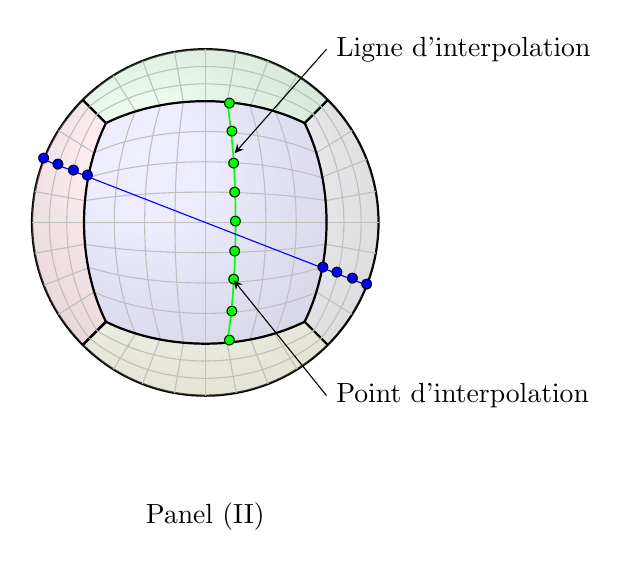
\begin{tikzpicture}[scale=2.2]
	\draw [line width=0.8pt] (0,0) circle (1cm);
    \shade[ball color=blue!10!white,opacity=0.20] (0,0) circle (1cm);	
	
	\filldraw[draw=black,fill=blue!30!white,opacity=0.20]
	plot [smooth,domain=-35:35] ({0.7*cos(\x)},{sin(\x)})
	-- plot [smooth,domain=55:125] ({cos(\x)},{0.7*sin(\x)})
	-- plot [smooth,domain=150:215] ({0.7*cos(\x)},{sin(\x)})
	-- plot [smooth,domain=240:300] ({cos(\x)},{0.7*sin(\x)})
	-- cycle;	
	\draw [samples=100,domain=48:132, color=gray!50] plot({cos(\x)},{0.35*sin(\x)});
	\draw [samples=100,domain=48:132, color=gray!50] plot({cos(\x)},{-.35*sin(\x)});
	\draw [samples=100,domain=46:134, color=gray!50] plot({cos(\x)},{0.175*sin(\x)});
	\draw [samples=100,domain=46:134, color=gray!50] plot({cos(\x)},{-.175*sin(\x)});
	\draw [samples=100,domain=50:130, color=gray!50] plot({cos(\x)},{0.525*sin(\x)});
	\draw [samples=100,domain=50:130, color=gray!50] plot({cos(\x)},{-.525*sin(\x)});
	\draw [samples=100,domain=45:135, color=gray!50] plot({cos(\x)},{0*sin(\x)});

	\draw [rotate=90, samples=100,domain=48:132, color=gray!50] plot({cos(\x)},{0.35*sin(\x)});
	\draw [rotate=90, samples=100,domain=48:132, color=gray!50] plot({cos(\x)},{-.35*sin(\x)});
	\draw [rotate=90, samples=100,domain=46:134, color=green, line width=0.6pt] plot({cos(\x)},{-.175*sin(\x)});
	\draw [rotate=90, samples=100,domain=46:134, color=gray!50] plot({cos(\x)},{0.175*sin(\x)});
	\draw [rotate=90, samples=100,domain=50:130, color=gray!50] plot({cos(\x)},{0.525*sin(\x)});
	\draw [rotate=90, samples=100,domain=50:130, color=gray!50] plot({cos(\x)},{-.525*sin(\x)});
	\draw [rotate=90, samples=100,domain=45:135, color=gray!50] plot({cos(\x)},{0*sin(\x)});

	\filldraw[draw=black,fill=red!30!white,opacity=0.20]
	plot [smooth,domain=145:215] ({.7*cos(\x)},{sin(\x)})
	-- plot [smooth] (-.573,-.573) -- (-.707,-.707)
	-- plot [smooth,domain=215:145] ({cos(\x)},{sin(\x)})
	-- plot [smooth] (-.707,.707) -- (-.573,.573)
	-- cycle;	
	\draw [line width=0.8pt] (-.573,-.573) -- (-.707,-.707) ;
	\draw [line width=0.8pt] (-.573,.573) -- (-.707,.707) ;
	\draw [color=gray!50] (-.669,.260) -- (-.9321,.3622) ;
	\draw [color=gray!50] (-.669,-.260) -- (-.9321,-.3622) ;
	\draw [color=gray!50] (-.6946,.1259) -- (-.9840,.1783) ;
	\draw [color=gray!50] (-.6946,-.1259) -- (-.9840,-.1783) ;
	\draw [color=gray!50] (-.6427,.4022) -- (-.8477,.5305) ;
	\draw [color=gray!50] (-.6427,-.4022) -- (-.8477,-.5305) ;
	\draw [color=gray!50] (-.707,0) -- (-1,0) ;
	\draw [samples=100,domain=141:219, color=gray!50] plot({0.8*cos(\x)},{sin(\x)});
	\draw [samples=100,domain=138:222, color=gray!50] plot({0.9*cos(\x)},{sin(\x)});
	
	\filldraw[draw=black,fill=green!30!white,opacity=0.20]
	plot [smooth,domain=55:125] ({cos(\x)},{0.7*sin(\x)})
	-- plot [smooth] (-.573,.573) -- (-.707,.707)
	-- plot [smooth,domain=125:55] ({cos(\x)},{sin(\x)})
	-- plot [smooth] (.707,.707) -- (.573,.573)
	-- cycle;	
	\draw [line width=0.8pt] (-.573,.573) -- (-.707,.707) ;
	\draw [line width=0.8pt] (.707,.707) -- (.573,.573) ;
	\draw [rotate=-90,color=gray!50] (-.669,.260) -- (-.9321,.3622) ;
	\draw [rotate=-90,color=gray!50] (-.669,-.260) -- (-.9321,-.3622) ;
	\draw [rotate=-90,color=gray!50] (-.6946,.1259) -- (-.9840,.1783) ;
	\draw [rotate=-90,color=gray!50] (-.6946,-.1259) -- (-.9840,-.1783) ;
	\draw [rotate=-90,color=gray!50] (-.6427,.4022) -- (-.8477,.5305) ;
	\draw [rotate=-90,color=gray!50] (-.6427,-.4022) -- (-.8477,-.5305) ;
	\draw [rotate=-90,color=gray!50] (-.707,0) -- (-1,0) ;
	\draw [rotate=-90,samples=100,domain=141:219, color=gray!50] plot({0.8*cos(\x)},{sin(\x)});
	\draw [rotate=-90,samples=100,domain=138:222, color=gray!50] plot({0.9*cos(\x)},{sin(\x)});
	
	\filldraw[draw=black,fill=yellow!30!white,opacity=0.20]
	plot [smooth,domain=55:125] ({cos(\x)},{-.7*sin(\x)})
	-- plot [smooth] (-.573,-.573) -- (-.707,-.707)
	-- plot [smooth,domain=125:55] ({cos(\x)},{-sin(\x)})
	-- plot [smooth] (.707,-.707) -- (.573,-.573)
	-- cycle;	
	\draw [line width=0.8pt] (-.573,-.573) -- (-.707,-.707) ;
	\draw [line width=0.8pt] (.707,-.707) -- (.573,-.573) ;
	\draw [rotate=90,color=gray!50] (-.669,.260) -- (-.9321,.3622) ;
	\draw [rotate=90,color=gray!50] (-.669,-.260) -- (-.9321,-.3622) ;
	\draw [rotate=90,color=gray!50] (-.6946,.1259) -- (-.9840,.1783) ;
	\draw [rotate=90,color=gray!50] (-.6946,-.1259) -- (-.9840,-.1783) ;
	\draw [rotate=90,color=gray!50] (-.6427,.4022) -- (-.8477,.5305) ;
	\draw [rotate=90,color=gray!50] (-.6427,-.4022) -- (-.8477,-.5305) ;
	\draw [rotate=90,color=gray!50] (-.707,0) -- (-1,0) ;
	\draw [rotate=90,samples=100,domain=141:219, color=gray!50] plot({0.8*cos(\x)},{sin(\x)});
	\draw [rotate=90,samples=100,domain=138:222, color=gray!50] plot({0.9*cos(\x)},{sin(\x)});
	
	\draw [rotate=180,color=gray!50] (-.669,.260) -- (-.9321,.3622) ;
	\draw [rotate=180,color=gray!50] (-.669,-.260) -- (-.9321,-.3622) ;
	\draw [rotate=180,color=gray!50] (-.6946,.1259) -- (-.9840,.1783) ;
	\draw [rotate=180,color=gray!50] (-.6946,-.1259) -- (-.9840,-.1783) ;
	\draw [rotate=180,color=gray!50] (-.6427,.4022) -- (-.8477,.5305) ;
	\draw [rotate=180,color=gray!50] (-.6427,-.4022) -- (-.8477,-.5305) ;
	\draw [rotate=180,color=gray!50] (-.707,0) -- (-1,0) ;
	\draw [rotate=180,samples=100,domain=141:219, color=gray!50] plot({0.8*cos(\x)},{sin(\x)});
	\draw [rotate=180,samples=100,domain=138:222, color=gray!50] plot({0.9*cos(\x)},{sin(\x)});
	
	\draw [samples=100,domain=55:125, line width=0.8pt] plot({cos(\x)},{0.7*sin(\x)});
	\draw [samples=100,domain=55:125, line width=0.8pt] plot({cos(\x)},{-.7*sin(\x)});
	\draw [samples=100,domain=145:215, line width=0.8pt] plot({.7*cos(\x)},{sin(\x)}); 
	\draw [samples=100,domain=145:215, line width=0.8pt] plot({-.7*cos(\x)},{sin(\x)}); 
	
	\draw (.175,0) node[color=green] {$\bullet$} ;
	\draw (.175,0) node {$\circ$} ;
	\draw (.17,.17) node[color=green] {$\bullet$} ;
	\draw (.17,.17) node {$\circ$} ;
	\draw (.165,.335) node[color=green] {$\bullet$} ;
	\draw (.165,.335) node {$\circ$} ;
	\draw (.155,.52) node[color=green] {$\bullet$} ;
	\draw (.155,.52) node {$\circ$} ;
	\draw (.14,.684) node[color=green] {$\bullet$} ;
	\draw (.14,.684) node {$\circ$} ;
	\draw (.17,-.17) node[color=green] {$\bullet$} ;
	\draw (.17,-.17) node {$\circ$} ;
	\draw (.165,-.335) node[color=green] {$\bullet$} ;
	\draw (.165,-.335) node {$\circ$} ;
	\draw (.155,-.52) node[color=green] {$\bullet$} ;
	\draw (.155,-.52) node {$\circ$} ;
	\draw (.14,-.684) node[color=green] {$\bullet$} ;
	\draw (.14,-.684) node {$\circ$} ;
	
	\draw [>=stealth, <-] (0.17,.4) -- (.7,1) ;
	\draw  (0.7,1) node[right] {Ligne d'interpolation} ;
	\draw [>=stealth, <-] (.165,-.335) -- (.7,-1) ;
	\draw  (0.7,-1) node[right] {Point d'interpolation} ;
	
	
	
	
	
	
	\draw [color=blue] (-.9321,.3622) -- (.9321,-.3622) ;
	\draw  (-.9321,.3622) node[color=blue] {$\bullet$} ;
	\draw (-.9321,.3622) node {$\circ$} ;	
	\draw  (.9321,-.3622) node[color=blue] {$\bullet$} ;
	\draw (.9321,-.3622) node {$\circ$} ;
	\draw  (-.85,0.3886*.85) node[color=blue] {$\bullet$} ;
	\draw (-.85,0.3886*.85) node {$\circ$} ;	
	\draw (.85,-0.3886*.85) node[color=blue] {$\bullet$} ;
	\draw (.85,-0.3886*.85) node {$\circ$} ;	
	\draw  (-.76,0.3886*.76) node[color=blue] {$\bullet$} ;
	\draw (-.76,0.3886*.76) node {$\circ$} ;	
	\draw (.76,-0.3886*.76) node[color=blue] {$\bullet$} ;
	\draw (.76,-0.3886*.76) node {$\circ$} ;
	\draw  (-.68,0.3886*.68) node[color=blue] {$\bullet$} ;
	\draw (-.68,0.3886*.68) node {$\circ$} ;	
	\draw (.68,-0.3886*.68) node[color=blue] {$\bullet$} ;
	\draw (.68,-0.3886*.68) node {$\circ$} ;	
	\draw (-.52,0.3886*.52) node[color=blue] {\begin{tiny}$\blacksquare$ \end{tiny}} ;
	\draw (-.52,0.3886*.52) node {\begin{tiny}$\square$ \end{tiny}} ;
	\draw (.52,-0.3886*.52) node[color=blue] {\begin{tiny}$\blacksquare$ \end{tiny}} ;
	\draw (.52,-0.3886*.52) node {\begin{tiny}$\square$ \end{tiny}} ;
	\draw (-.36,0.3886*.36) node[color=blue] {\begin{tiny}$\blacksquare$ \end{tiny}} ;
	\draw (-.36,0.3886*.36) node {\begin{tiny}$\square$ \end{tiny}} ;
	\draw (.36,-0.3886*.36) node[color=blue] {\begin{tiny}$\blacksquare$ \end{tiny}} ;
	\draw (.36,-0.3886*.36) node {\begin{tiny}$\square$ \end{tiny}} ;
	\draw (-.18,0.3886*.18) node[color=blue] {\begin{tiny}$\blacksquare$ \end{tiny}} ;
	\draw (-.18,0.3886*.18) node {\begin{tiny}$\square$ \end{tiny}} ;
	\draw (.18,-0.3886*.18) node[color=blue] {\begin{tiny}$\blacksquare$ \end{tiny}} ;
	\draw (.18,-0.3886*.18) node {\begin{tiny}$\square$ \end{tiny}} ;
	\draw (0,0) node[color=blue] {\begin{tiny}$\blacksquare$ \end{tiny}} ;
	\draw (0,0) node {\begin{tiny}$\square$ \end{tiny}} ;
	
	\draw  (0,-1.7) node {Panel (II)} ;

\end{tikzpicture}
\end{center}
\caption{La ligne bleue représente une isoligne $\eta=\eta_j$ du panel $(I)$ vue depuis le panel $(II)$. les cercles bleus représentent des points de la Cubed-Sphere contenues dans l'isoligne $\eta=\eta_j$, les carrés bleus sont des points de l'isoligne $\eta=\eta_j$ qui ne sont pas sur la Cubed-Sphere. En vert, une portion du grand cercle utilisé pour l'interpolation.}
\label{fig: panel II_interp2}
\end{figure}  

Le procédé est symétrique pour reconstruire les données sur un grand cercle $C_i^{(1)}$ ou le grand cercle d'un autre panel.
Une fois les données $(f_p)_{0 \leq p \leq 4N-1}$ construites, on peut calculer l'approximation de la dérivée grâce à $\partial_{\xi} f_p \approx \delta_{\Delta \xi}^H f_p$
que l'on restreint aux points du maillage par 
\begin{equation}
\left\lbrace
\begin{array}{rcl}
f_{\xi,i,j}^{(I)} & = & \delta_{4, \xi}^H f_{i-N/2}\\
f_{\xi,i,j}^{(III)} & = & \delta_{4, \xi}^H f_{i+3N/2}
\end{array}
\right.
\text{ pour } C^{(2)}_j \text{ fixé.}
\end{equation}

Finalement, le procédé total de calcul des dérivées hermitienne est $\xi$ sur un panel $k$ est donné par l'algorithme \ref{alg:deltaxi}.

\begin{center}
\begin{minipage}[H]{12cm}
  \begin{algorithm}[H]
    \caption{: Calcul de $f_{\xi, i, j}^{(I)}$ et $f_{\xi, i, j}^{(III)}$}\label{alg:deltaxi}
    \begin{algorithmic}[1]
    \For{ $j=-N/2, \ldots , N/2$, }
    \State pour un grand cercle $C_j^{(2)}$ fixé,
    \For{$p=0,1, \ldots 4N-1$ définir les points $\mathbf{m}_p$ du grand cercle bleu}
             \State  $\mathbf{m}_p = \mathbf{m}_{p-N/2,j}^{(I)}$ pour $0  \leq p \leq N$ donc $f_p = f(\mathbf{m}_p)$,
             \State $f_p = P_{C_p}(\mathbf{m}_p)$, où $P_{C_p}$ est la fonction d'interpolation utilisant les points de l'isoligne $\xi = \xi^{(II)}_{p-N/2+1}$ pour $N+1 \leq p \leq 2N-1$,
             \State  $\mathbf{m}_p = \mathbf{m}_{p-3N/2,j}^{(III)}$ pour $2N  \leq p \leq 3N-1$ donc $f_p = f(\mathbf{m}_p)$,
             \State $f_p = P_{C_p}(\mathbf{m}_p)$, où $P_{C_p}$ est la fonction d'interpolation utilisant les points de l'isoligne $\xi = \xi^{(VI)}_{p-3N/2+1}$ pour $3N+1 \leq p \leq 4N-1$.
            \EndFor
    \State Calcul de $\delta_{4, \xi}^H f_p$,
    \State Affectation $f_{\xi,i,j}^{(I)} = \delta_{4, \xi}^H f_{i+N/2}$,
    \State Affectation $f_{\xi,i,j}^{(III)} = \delta_{4, \xi}^H f_{i+3N/2}$.
    \EndFor
    \end{algorithmic}
    \end{algorithm}
\end{minipage}
\end{center}
De la même manière, l'algorithme de construction des dérivées approchées en $\eta$ sur les panels $(I)$ et $(III)$ est l'algorithme \ref{alg:deltaeta}.
\begin{center}
\begin{minipage}[H]{12cm}
  \begin{algorithm}[H]
    \caption{: Calcul de $f_{\eta, i, j}^{(I)}$ et $f_{\eta, i, j}^{(III)}$}\label{alg:deltaeta}
    \begin{algorithmic}[1]
    \For{ $i=-N/2, \ldots , N/2$, }
    \State pour un grand cercle $C_i^{(1)}$ fixé,
    \For{$p=0,1, \ldots 4N-1$ définir les points $\mathbf{m}_p$}
             \State  $\mathbf{m}_p = \mathbf{m}_{i,p-N/2}^{(I)}$ pour $0  \leq p \leq N$ donc $f_p = f(\mathbf{m}_p)$,
             \State $f_p = P_{C_p}(\mathbf{m}_p)$, où $P_{C_p}$ est la fonction d'interpolation utilisant les points de l'isoligne $\eta = \eta^{(V)}_{p-N/2+1}$ pour $N+1 \leq p \leq 2N-1$,
             \State  $\mathbf{m}_p = \mathbf{m}_{i,5N/2-p}^{(III)}$ pour $2N  \leq p \leq 3N-1$ donc $f_p = f(\mathbf{m}_p)$ (Attention à l'orientation sur les panels),
             \State $f_p = P_{C_p}(\mathbf{m}_p)$, où $P_{C_p}$ est la fonction d'interpolation utilisant les points de l'isoligne $\eta = \eta^{(VI)}_{p-3N/2+1}$ pour $3N+1 \leq p \leq 4N-1$.
            \EndFor
    \State Calcul de $\delta_{4, \eta}^H f_p$,
    \State Affectation $f_{\eta,i,j}^{(I)} = \delta_{4, \eta}^H f_{i+N/2}$,
    \State Affectation $f_{\eta,i,j}^{(III)} = \delta_{4, \eta}^H f_{i+3N/2}$.
    \EndFor
    \end{algorithmic}
    \end{algorithm}
\end{minipage}
\end{center}
Le processus est utilisé sur chaque panel $(k) = (I), \ldots , (VI)$. On obtient alors les approximations des dérivées en $\xi$ et en $\eta$ sur chaque point du maillage Cubed-Sphere $\mathbf{x}_{i,j}^{(k)}$ avec $-N/2 \leq i,j \leq N/2$.

\begin{theoreme}
Pour tous $-N/2 \leq i,j \leq N/2$ et $(k) = (I) , \ldots , (VI)$ et pour $f : \mathbf{x} \in \mathbb{S}_a^2 \mapsto f(\mathbf{x}) \in \mathbb{R}$ une fonction régulière, on a 
\begin{equation}
\left\lbrace
\begin{array}{rcl}
f_{\xi,i,j}^{(k)} & = & \partial_{\xi} f(\mathbf{x}_{i,j}^{(k)}) + \mathcal{O}(\Delta \eta^3) \\
f_{\eta,i,j}^{(k)} & = & \partial_{\eta} f(\mathbf{x}_{i,j}^{(k)}) + \mathcal{O}(\Delta \xi^3)
\end{array}
\right.
\end{equation}
\label{th:consistance_der_xieta}
\end{theoreme}

\begin{proof}
La preuve est la même sur chaque panel, on se concentre ici sur le panel $(I)$. De plus, par symétrie, nous ne montrons que le premier résultat :
\begin{equation}
f_{\xi,i,j}^{(k)} = \partial_{\xi} f(\mathbf{x}_{i,j}^{(k)}) + \mathcal{O}(\Delta \eta^3)
\end{equation}
Le procédé de construction des valeur sur un grand cercle $C_j^{(2)}$, aux points $\mathbf{m}_p$ avec $0 \leq p \leq 4N-1$, nous donne le résultat
\begin{equation}
f_p = f(\mathbf{m}_p) + \mathcal{O}(\Delta \eta^4)
\end{equation}
Donc dans le calcul effectif de la dérivée Hermitienne, on a 
\begin{equation}
\delta_{2,\xi} f_p = \dfrac{f_{p+1} - f_{p-1}}{2 \Delta \xi} = \dfrac{f(\mathbf{m}_{p+1}) - f(\mathbf{m}_{p-1})}{2 \Delta \xi} + \mathcal{O}\left( \dfrac{\Delta \eta^4}{\Delta \xi} \right).
\end{equation}
On considère que sur la Cubed-Sphere $\Delta \xi = \Delta \eta$. Alors en composant par $\sigma_{\xi}^{-1}$, on a 
\begin{align*}
\delta_{4,\xi}^H f_p & = \sigma_{\xi}^{-1} \circ \delta_{2,\xi} f_p \\
                   & = \sigma_{\xi}^{-1} \circ \left( \dfrac{f(\mathbf{m}_{p+1}) - f(\mathbf{m}_{p-1})}{2 \Delta \xi} + \mathcal{O}\left( \Delta \eta^3 \right) \right)\\
                   & = \sigma_{\xi}^{-1} \circ \left( \dfrac{f(\mathbf{m}_{p+1}) - f(\mathbf{m}_{p-1})}{2 \Delta \xi}\right)  + \mathcal{O}\left( \Delta \eta^3 \right) \\
                   & = \partial_{\xi}f(\mathbf{m}_p) + \mathcal{O}\left( \Delta \eta^3 \right) + \mathcal{O}\left( \Delta \xi^4 \right) \\
                   & = \partial_{\xi}f(\mathbf{m}_p) + \mathcal{O}\left( \Delta \eta^3 \right).\\
\end{align*}
On assigne les dérivées aux points des panels à l'aide de $\mathbf{m}_p=\mathbf{x}^{(k)}_{p-N/2,j}$ pour $p = 0 \ldots N$. Le résultat est alors :
\begin{equation}
f^{(k)}_{\xi,i,j} = \delta_{4,\xi}^H f_{i+N/2} = \partial_{\xi} f(\mathbf{x}^{(k)}_{i+N/2,j}) + \mathcal{O}\left( \Delta \eta^3 \right).
\end{equation}
Le résultat concernant la dérivée en $\eta$ est obtenu de la même manière.
\end{proof}

D'après le théorème \ref{th:consistance_der_xieta}, la méthode de calcul est d'ordre au moins 3. Cependant, on note que l'interpolation (qui empêche la méthode d'être d'ordre 4) n'intervient qu'en dehors des panels où l'on souhaite calculer la dérivée.
Lorsque l'on souhaite calculer une approximation de $\partial_{\xi}f(\mathbf{x}_{i,j}^{(I)})$, l'interpolation intervient sur les panels $(II)$ et $(IV)$ mais pas sur le panel $(I)$. Dans la pratique, on s'attend à ce que la méthode soit d'ordre $4$, en particulier loin des bords des panels.









\subsection{Opérateur gradient discret}

Soit $h : \mathbf{x} \in \mathbb{S}_a^2 \mapsto h(\mathbf{x}) \in \mathbb{R}$ une fonction régulière sur la Sphère. On note $h_{i,j}^{(k)} = h(\mathbf{x}_{i,j}^{(k)})$, avec $-N/2 \leq i,j \leq N/2$ et $(k) = (I) , \ldots , (VI)$, la valeur de $h$ au point $\mathbf{x}_{i,j}^{(k)}$ de la Cubed-Sphere.
Nous notons $( \mathbf{g}^{\xi} )_{i,j}^{(k)} = \mathbf{g}^{\xi} (\mathbf{x}_{i,j}^{(k)})$ et $( \mathbf{g}^{\eta} )_{i,j}^{(k)} = \mathbf{g}^{\eta} (\mathbf{x}_{i,j}^{(k)})$.

\begin{definition}
On définit l'opérateur \textit{gradient discret} par 
\begin{equation}
\nabla_{T,\Delta} h_{i,j}^{(k)} = h_{\xi,i,j}^{(k)} ( \mathbf{g}^{\xi} )_{i,j}^{(k)} + h_{\eta,i,j}^{(k)} ( \mathbf{g}^{\eta} )_{i,j}^{(k)}
\end{equation}
avec $-N/2 \leq i,j \leq N/2$ et $(k) = (I), \ldots , (VI)$ ainsi que $h_{\xi,i,j}^{(k)}$ et $h_{\eta,i,j}^{(k)}$ obtenus grâce aux algorithmes \ref{alg:deltaxi} et \ref{alg:deltaeta}.
\label{def:gradient_disc}
\end{definition}
L'opérateur gradient discret de $h$, $\nabla_{T,\Delta} h_{i,j}^{(k)}$ donne une approximation du gradient continu en $\mathbf{x}_{i,j}^{(k)}$. En effet, le résultat de consistance suivant est vérifié:

\begin{proposition}
Soit $h : \mathbf{x} \in \mathbb{S}_a^2 \mapsto h(\mathbf{x}) \in \mathbb{R}$ une fonction régulière sur la Sphère. Pour tous $-N/2 \leq i,j \leq N/2$ et $(k)=(I), \ldots , (VI)$, on a
\begin{equation}
\nabla_{T,\Delta} h_{i,j}^{(k)} - (\nabla_T h)^{*,(k)}_{i,j} = \mathcal{O} \left( \Delta^3 \right)
\end{equation}
où $^*$ désigne la restriction à la Cubed-Sphere et $\Delta = \Delta \xi = \Delta \eta$. 
\label{prop:accuracy_gradient}
\end{proposition}

\begin{proof}
Ce résultat est une conséquence immédiate de la linéarité du gradient discret et du théorème \ref{th:consistance_der_xieta}.
\end{proof}
De plus, on note que par construction
\begin{equation}
\nabla_{T,\Delta} h_{i,j}^{(k)} \in \mathbb{T}_{\mathbf{x}_{i,j}^{(k)}} \mathbb{S}_a^2.
\end{equation}
Une valeur du gradient est associée à chaque point de chaque panel, lorsque le point appartient à plusieurs panels, la moyenne des gradients est conservée.




Une fois l'opérateur d'approximation du gradient définit, il faut le tester numériquement pour tester son comportement. On se donne $h$ tel que le gradient $\nabla_T h$ est connue et nous comparons le gradient approché et le gradient exacte.
Si $h$ est une fonction sphérique, on sait que $h$ se décompose comme une somme d'harmoniques sphériques. De plus, les harmoniques sphériques sont des restrictions de polynômes sur la Sphère $\mathbb{S}_a^2$. Un test pertinent est donc de choisir $h$ de la forme
\begin{equation}
\left\lbrace
\begin{array}{rcl}
\hat{h}(x,y,z) & = & x^p y^q z^r, \\
h & = & \hat{h}_{| \mathbb{S}_a^2}.
\end{array}
\right.
\label{eq:grad_test}
\end{equation}
Avec $p, q, r \in \mathbb{N}$.
En se basant sur la proposition \ref{prop:gradient_project}, on peut facilement déterminer le gradient de $h$ par
\begin{equation}
\nabla_T h = \nabla_{\mathbb{R}^3} \hat{h} - \mathbf{n} \left( \mathbf{n} \cdot \nabla_{\mathbb{R}^3} \hat{h} \right)
\end{equation}
avec $\mathbf{n} = \mathbf{x}/a$ la normale extérieure en $\mathbf{x} \in \mathbb{S}_a^2$ et $\nabla_{\mathbb{R}^3} \hat{h}$ donné dans la base $(\mathbf{i}, \mathbf{j}, \mathbf{k})$ par 
\begin{align*}
\nabla_{\mathbb{R}^3} \hat{h} & = \dfrac{\partial \hat{h}}{\partial x} \mathbf{i} + \dfrac{\partial \hat{h}}{\partial y} \mathbf{j} + \dfrac{\partial \hat{h}}{\partial z} \mathbf{k}\\
                              & = p x^{p-1} y^q z^r \mathbf{i} + q x^p y^{q-1} z^r \mathbf{j} + r x^p y^q z^{r-1} \mathbf{k}.
\end{align*}
Si $\mathbf{u}$ est une fonction vectorielle définit sur la Cubed-Sphere, alors
\begin{equation}
\mathbf{u}_{i,j}^{(k)} = u_{i,j}^{(k)} \mathbf{i} + v_{i,j}^{(k)} \mathbf{j} + w_{i,j}^{(k)} \mathbf{k}
\end{equation}
On définit la norme $\mathcal{N}$ par
\begin{equation}
\mathcal{N}(\mathbf{u}) = \max_{-N/2 \leq i,j \leq N/2} \max_{(k) = (I) \ldots (VI)} \max (u_{i,j}^{(k)}, v_{i,j}^{(k)}, w_{i,j}^{(k)}).
\end{equation}
On mesure l'erreur faite sur le calcul du gradient approché par
\begin{equation}
e_{\Delta} = \dfrac{\mathcal{N}\left(\nabla_{T,\Delta}h - \left( \nabla_{T}h \right)^* \right)}{\mathcal{N}\left(\left( \nabla_{T}h \right)^* \right)}
\end{equation}
Dans la figure \ref{fig:rate_grad}, on trace le logarithme décimal de l'erreur en fonction du logarithme décimal de $\frac{\pi a}{2 N} = a \Delta \xi = a \Delta \eta$. La pente de cette courbe nous donne l'ordre de convergence de la méthode sur le test effectué.

\begin{figure}[htbp]
\begin{center}
\includegraphics[height=5cm]{rate_grad_1_123.png}
\includegraphics[height=5cm]{rate_grad_1_222.png}
\end{center}
\caption{Convergence du gradient de \eqref{eq:grad_test} avec $(p,q,r)=(1,2,3)$ à gauche et avec $(p,q,r)=(2,2,2)$ à droite.}
\label{fig:rate_grad}
\end{figure}

Les ordres estimés sont meilleurs que l'ordre 3 montré dans la proposition \ref{prop:accuracy_gradient}. Lorsque $(p,q,r)=(1,2,3)$, l'ordre de convergence calculé est $3.8787$, il est de $3.8868$ lorsque $(p,q,r)=(2,2,2)$. Cela confirme l'ordre démontré et nous donne un ordre proche de $4$ dans la pratique. Les erreurs effectives sont données en fonction de $N$ dans la table \ref{tab:rate_grad}.

\begin{table}[htbp]
\begin{center}
\begin{tabular}{|c||c|c|}
\hline
$\mathbf{N}$    & $\mathbf{(1,2,3)}$     & $\mathbf{(2,2,2)}$     \\
\hline
\hline
$16$   & $1.8636 (-4)$ & $3.1368 (-4)$ \\
$32$   & $1.3545 (-5)$ & $2.3910 (-5)$ \\
$64$   & $9.7564 (-7)$ & $1.6716 (-6)$ \\
$128$  & $6.5592 (-8)$ & $1.1088 (-7)$ \\
$256$  & $4.2563 (-9)$ & $7.1437 (-9)$ \\
$511$  & $2.7115(-10)$ & $4.5361(-10)$ \\
\hline
\hline
\textbf{ordre estimé} & $3.8787$ & $3.8868$ \\
\hline 
\end{tabular}
\end{center}
\caption{Table de convergence du gradient approché de \eqref{eq:grad_test} avec $(p,q,r)=(1,2,3)$ à gauche et avec $(p,q,r)=(2,2,2)$ à droite.}
\label{tab:rate_grad}
\end{table}















\subsection{Variante de l'opérateur de gradient discret}


\subsubsection{Gradient discret utilisant un schéma compact d'ordre 8}

Une variante pour la calcul du gradient approché est d'utiliser un schéma aux différences finies 1D d'ordre plus élevé que $\delta_{4,x}^H$ (qui est d'ordre 4). 
L'opérateur centré hermitien $\delta_{8,x}^H$ est un opérateur d'approximation de la dérivée première à l'ordre $8$.
On remplace $\delta_{4, \xi}^H$ et $\delta_{4, \eta}^H$ dans les algorithmes \ref{alg:deltaxi} et \ref{alg:deltaeta} de calcul de dérivées sur les grands cercles par $\delta_{8, \xi}^H$ et $\delta_{8, \eta}^H$, le reste étant inchangé. Le nouveau gradient approché vérifie toujours la proposition \ref{prop:accuracy_gradient}, le facteur limitant la montée en ordre étant la fonction d'interpolation.

Dans la figure \ref{fig:rate_grad2}, nous présentons les courbes de convergence comparant le schéma utilisant $\delta^H_{4,x}$ et $\delta^H_{8,x}$. On constate que le premier schéma est meilleur en ordre que le schéma utilisant $\delta^H_{8,x}$. En revanche, l'erreur pour des $N$ plus faible est bien meilleure pour le schéma utilisant $\delta^H_{8,x}$ comme on peut le voir dans le tableau \ref{tab:rate_grad2}.

\begin{figure}[htbp]
\begin{center}
\includegraphics[height=5cm]{rate_grad_2_123.png}
\includegraphics[height=5cm]{rate_grad_2_222.png}
\end{center}
\caption{Convergence du gradient de \eqref{eq:grad_test} avec $(p,q,r)=(1,2,3)$ à gauche et avec $(p,q,r)=(2,2,2)$ à droite. Nous comparons l'utilisation de $\delta^H_{4,x}$ en magenta avec l'utilisation de $\delta^H_{8,x}$ en bleu.}
\label{fig:rate_grad2}
\end{figure}


\begin{table}[htbp]
\begin{center}
\begin{tabular}{|c||c|c||c|c|}
\hline
  & \multicolumn{2}{c||}{$\mathbf{(p,q,r)=(1,2,3)}$} & \multicolumn{2}{c|}{$\mathbf{(p,q,r)=(2,2,2)}$} \\
\hline
$\mathbf{N}$    &  $\delta^H_{4,x}$  & $\delta^H_{8,x}$  &  $\delta^H_{4,x}$  & $\delta^H_{8,x}$     \\
\hline
\hline
$16$   & $1.8636 (-4)$ & $1.8475 (-5)$ & $3.1368 (-4)$ & $3.1349 (-5)$ \\
$32$   & $1.3545 (-5)$ & $2.0130 (-6)$ & $2.3910 (-5)$ & $3.4020 (-6)$ \\
$64$   & $9.7564 (-7)$ & $2.1919 (-7)$ & $1.6716 (-6)$ & $3.9216 (-7)$ \\
$128$  & $6.5592 (-8)$ & $2.4346 (-8)$ & $1.1088 (-7)$ & $4.7945 (-8)$ \\
$256$  & $4.2563 (-9)$ & $2.9159 (-9)$ & $7.1437 (-9)$ & $3.8473 (-9)$ \\
$511$  & $2.7115(-10)$ & $3.5643 (-10)$& $4.5361(-10)$ & $7.2161(-10)$ \\
\hline
\hline
\textbf{ordre estimé} & $3.8787$ & $3.1363$ & $3.8868$ & $3.1266$\\
\hline 
\end{tabular}
\end{center}
\caption{Table de convergence du gradient approché de \eqref{eq:grad_test} utilisant $\delta^H_{8,x}$ ou $\delta^H_{x}$.}
\label{tab:rate_grad2}
\end{table}

Dans la figure \ref{fig:err_grad}, nous représentons l'erreur spatiale
\begin{equation}
\mathbf{x}_{i,j}^{(k)} \mapsto \dfrac{\max_{\mathbf{u}=\mathbf{i}, \mathbf{j}, \mathbf{k}} | \left( \nabla_{T,app} h_{i,j}^{(k)} - \nabla_T h_{i,j}^{(k)} \right)\cdot \mathbf{u}_{i,j}^{(k)} | }{\max_{\mathbf{u}=\mathbf{i}, \mathbf{j}, \mathbf{k}} \left(  | \nabla_T h_{i,j}^{(k)} |\right)\cdot \mathbf{u}_{i,j}^{(k)}}
\end{equation}
où $\nabla_{T,app} h_{i,j}^{(k)}$ désigne le gradient approché calculé en utilisant $\delta_{8,x}^H$ la dérivée Hermitienne d'ordre 8 et $\mathbf{x}_{i,j}^{(k)}$ est un point de la Cubed-Sphere, $(k)= (I), \ldots , (VI)$ et $-N/2 \leq i,j \leq N/2$.
\begin{figure}[htbp]
\begin{center}
\includegraphics[scale=0.5]{snap_grad_err8.png}
\end{center}
\caption{Erreur relative pour le calcul du gradient $\nabla_{T,app} h_{i,j}^{(k)}$ avec $N=63$ et $h(x,y,z)=x y^2 z^3$. }
\label{fig:err_grad}
\end{figure}
On observe que l'erreur est concentrée là où l'interpolation est la plus mauvaise. Sur les grands cercles associées aux isolignes $\xi = \pm \frac{\pi}{4}$ ou $\eta = \pm \frac{\pi}{4}$ ou $\xi = 0$ ou $\eta = 0$, il n'y a pas d'interpolation car ces grands cercles passent exactement à des points de grilles sur tous les panels. Il s'agit des grands cercles passant par sur les bords de panels ainsi que ceux centraux sur les panels. L'erreur introduite par l'interpolation est particulièrement visible loin de ces cercles.













\subsubsection{Gradient sans interpolation}

Nous avons vu que la méthode de calcul du gradient approché repose sur le calcul de dérivées hermitiennes périodique le long de grands cercles. L'utilisation de splines cubiques empêche de passer à un ordre supérieur à 3 en changeant l'ordre de la dérivée Hermitienne. Dans cette sous section, nous utilisons un schéma décentré à proximité du bord de manière à n'utiliser que les points intérieurs du panel $(k)$ pour calculer le gradient en $\mathbf{x}_{i,j}^{(k)}$ avec $(k) = (I), \ldots ,(VI)$ et $-N/2 \leq i,j \leq N/2$.

Soit $(\mathfrak{u}_p)_{-N/2 \leq p \leq N/2}$ une fonction de grille. On définit l'opérateur explicite $\delta_{\dec,x}$ par
\begin{equation}
\left\lbrace
\begin{array}{rcll}
\delta_{\dec,x} \mathfrak{u}_p & = & \dfrac{1}{2 h} (\mathfrak{u}_{p+1}-\mathfrak{u}_{p-1}) & \text{ si } -N/2+1 \leq p \leq N/2-1 \\
\delta_{\dec,x} \mathfrak{u}_p & = & \dfrac{1}{h} \left( -\dfrac{103}{72} \mathfrak{u}_p + \dfrac{91}{36} \mathfrak{u}_{p+1} - \dfrac{7}{4} \mathfrak{u}_{p+2} + \dfrac{29}{36} \mathfrak{u}_{p+3} - \dfrac{11}{72} \mathfrak{u}_{p+4} +\right) & \text{ si } p = -N/2 \\
\delta_{\dec,x} \mathfrak{u}_p & = & \dfrac{1}{h} \left( \dfrac{103}{72} \mathfrak{u}_p - \dfrac{91}{36} \mathfrak{u}_{p+1} + \dfrac{7}{4} \mathfrak{u}_{p+2} - \dfrac{29}{36} \mathfrak{u}_{p+3} + \dfrac{11}{72} \mathfrak{u}_{p+4} +\right) & \text{ si } p = N/2 \\
\end{array}
\right.
\end{equation}
ainsi que l'opérateur $\sigma_{\dec,x}$ par
\begin{equation}
\left\lbrace
\begin{array}{rcll}
\delta_{\dec,x} \mathfrak{u}_p & = & \dfrac{1}{6} \mathfrak{u}_{p+1} + \dfrac{4}{6} \mathfrak{u}_{p} + \dfrac{1}{6} \mathfrak{u}_{p-1} & \text{ si } -N/2+1 \leq p \leq N/2-1 \\
\delta_{\dec,x} \mathfrak{u}_p & = & \dfrac{1}{6} \mathfrak{u}_{p-1} + \dfrac{4}{6} \mathfrak{u}_{p} & \text{ si } p = -N/2 \\
\delta_{\dec,x} \mathfrak{u}_p & = & \dfrac{4}{6} \mathfrak{u}_{p} + \dfrac{1}{6} \mathfrak{u}_{p-1} & \text{ si } p = N/2 \\
\end{array}
\right.
\end{equation}
L'opérateur hermitien $\delta^H_{\dec,x} = \sigma_{\dec,x}^{-1} \circ \delta_{\dec,x}$ est un opérateur d'approximation de la dérivée première d'ordre 4. Son décentrement au bord des panels permet d'obtenir une nouvelle procédure de calcul des dérivées $h_{\xi,i,j}$ et $h_{\eta,i,j}$ donnée par 
\begin{equation}
\left\lbrace
\begin{array}{rcll}
h_{\xi,i,j}^{(k)} & = & \delta^H_{\dec,\Delta \xi} h_{i,j}^{(k)} & j \text{ fixé,}\\
h_{\eta,i,j}^{(k)} & = & \delta^H_{\dec,\Delta \eta} h_{i,j}^{(k)} & i \text{ fixé.}
\end{array}
\right.
\end{equation}
Comme $\delta^H_{\dec,x}$ est un opérateur d'ordre $4$, le gradient approché donné par 
\begin{equation}
\nabla_{T,\dec} h_{i,j}^{(k)} = \delta^H_{\dec,\Delta \xi} h_{i,j}^{(k)} ( \mathbf{g}^{\xi} )_{i,j}^{(k)} + \delta^H_{\dec,\Delta \eta} h_{i,j}^{(k)} ( \mathbf{g}^{\eta} )_{i,j}^{(k)}
\end{equation}
est un gradient d'ordre 4.
Nous observons en figure \ref{fig:rate_grad3} la convergence de ce gradient $\nabla_{T,\dec} h_{i,j}^{(k)}$ en comparaison au gradient $\nabla_{T,\Delta} h_{i,j}^{(k)}$.
\begin{figure}[htbp]
\begin{center}
\includegraphics[height=5cm]{rate_grad_3_123.png}
\includegraphics[height=5cm]{rate_grad_3_222.png}
\end{center}
\caption{Convergence du gradient approché avec $(p,q,r)=(1,2,3)$ à gauche et avec $(p,q,r)=(2,2,2)$ à droite. Nous comparons le gradient $\nabla_{T,\dec}$ en bleu et le gradient $\nabla_{T,\Delta}$ en magenta.}
\label{fig:rate_grad3}
\end{figure}
Les ordres de convergence sont pratiquement les mêmes. Cependant, les erreurs à $N$ fixé sont bien plus faible pour $\nabla_{T,\Delta}$ qu'avec $\nabla_{T,\dec}$ comme on peut le voir dans la table \ref{tab:rate_grad3}.

\begin{table}[htbp]
\begin{center}
\begin{tabular}{|c||c|c||c|c|}
\hline
  & \multicolumn{2}{c||}{$\mathbf{(p,q,r)=(1,2,3)}$} & \multicolumn{2}{c|}{$\mathbf{(p,q,r)=(2,2,2)}$} \\
\hline
$\mathbf{N}$    &  $\nabla_{T,\Delta}$  & $\nabla_{T,\dec}$  &  $\nabla_{T,\Delta}$  & $\nabla_{T,\dec}$     \\
\hline
\hline
$16$   & $1.8636 (-4)$ & $5.0425 (-3)$ & $3.1368 (-4)$ & $1.1437 (-2)$ \\
$32$   & $1.3545 (-5)$ & $3.9160 (-4)$ & $2.3910 (-5)$ & $9.7399 (-4)$ \\
$64$   & $9.7564 (-7)$ & $3.1917 (-5)$ & $1.6716 (-6)$ & $6.6478 (-5)$ \\
$128$  & $6.5592 (-8)$ & $2.2341 (-6)$ & $1.1088 (-7)$ & $4.2363 (-6)$ \\
$256$  & $4.2563 (-9)$ & $1.4700 (-7)$ & $7.1437 (-9)$ & $2.6521 (-7)$ \\
$511$  & $2.7115(-10)$ & $9.4135 (-9)$ & $4.5361(-10)$ & $1.6554 (-8)$ \\
\hline
\hline
\textbf{ordre estimé} & $3.8787$ & $3.8036$ & $3.8868$ & $3.8997$\\
\hline 
\end{tabular}
\end{center}
\caption{Table de convergence des gradients approchés $\nabla_{T,\Delta}$ et $\nabla_{T,\dec}$.}
\label{tab:rate_grad3}
\end{table}














\subsection{Opérateur divergence discret}

Soit $\mathbf{v} : \mathbf{x} \in \mathbb{S}_a^2 \mapsto \mathbf{v}(\mathbf{x}) \in \mathbb{T}_{\mathbf{x}} \mathbb{S}_a^2$ un champ de vecteur régulier sur la sphère. Il existe alors $u$, $v$ et $w$ des fonctions régulières de $\mathbb{S}_a^2$ dans $\mathbb{R}$ telles que
\begin{equation}
\mathbf{v}(\mathbf{x}) = u(\mathbf{x}) \mathbf{i} + v (\mathbf{x}) \mathbf{j} + w(\mathbf{x}) \mathbf{k}
\end{equation}
avec $(\mathbf{i}, \mathbf{j}, \mathbf{k})$ la base canonique de $\mathbb{R}^3$ et $\mathbf{x} \in \mathbb{S}_a^2$. On définit $\mathbf{v}_{\xi,i,j}^{(k)}$ et $\mathbf{v}_{\eta,i,j}^{(k)}$ par
\begin{equation}
\left\lbrace
\begin{array}{rcl}
\mathbf{v}_{\xi,i,j}^{(k)} & = & u_{\xi,i,j}^{(k)} \mathbf{i} + v_{\xi,i,j}^{(k)} \mathbf{j} + w_{\xi,i,j}^{(k)} \mathbf{k} \\
\mathbf{v}_{\eta,i,j}^{(k)} & = & u_{\eta,i,j}^{(k)} \mathbf{i} + v_{\eta,i,j}^{(k)} \mathbf{j} + w_{\eta,i,j}^{(k)} \mathbf{k}
\end{array}
\right.
\text{ pour } -N/2 \leq  i,j \leq N/2 \text{, } (k) = (I), \ldots, (VI). 
\label{eq:der_partiel_vect}
\end{equation}
où les fonctions de grilles $(u_{\xi,i,j}^{(k)}), (u_{\eta,i,j}^{(k)}),  \ldots$ sont construites grâce aux algorithmes \ref{alg:deltaxi} et \ref{alg:deltaeta}.

\begin{definition}
On définit l'opérateur \textit{divergence discrète} par 
\begin{equation}
\nabla_{T,\Delta} \cdot \mathbf{v}_{i,j}^{(k)} = \mathbf{v}_{\xi,i,j}^{(k)} \cdot ( \mathbf{g}^{\xi} )_{i,j}^{(k)} + \mathbf{v}_{\eta,i,j}^{(k)} \cdot ( \mathbf{g}^{\eta} )_{i,j}^{(k)}
\end{equation}
avec $-N/2 \leq i,j \leq N/2$ et $(k) = (I), \ldots , (VI)$.
\label{def:divergence_disc}
\end{definition}
Comme pour le gradient, si un point $\mathbf{x}_{i,j}^{(k)}$ appartient à plusieurs panels, on y calcule plusieurs divergences. La moyenne des divergences est conservée en ce point.
L'opérateur divergence discret de $\mathbf{v}_{i,j}^{(k)}$ est une approximation du gradient en $\mathbf{x}_{i,j}^{(k)}$. En effet

\begin{proposition}
Soit $\mathbf{v} : \mathbf{x} \in \mathbb{S}_a^2 \mapsto \mathbf{v}(\mathbf{x}) \in \mathbb{T}_{\mathbf{x}} \mathbb{S}_a^2$ un champ de vecteur régulier sur la sphère. Alors pour tout $-N/2 \leq i,j \leq N/2$ et $(k) = (I) , \ldots , (VI)$, on a 
\begin{equation}
\nabla_{T,\Delta} \cdot \mathbf{v}_{i,j}^{(k)} - (\nabla_{T} \cdot \mathbf{v} )_{i,j}^{*,(k)} = \mathcal{O} \left( \Delta^3 \right)
\end{equation}
où $*$ désigne la restriction à la Cubed-Sphere et $\Delta  = \Delta \xi = \Delta \eta$.
\label{prop:accuracy_divergence}
\end{proposition}

\begin{proof}
Conséquence du théorème \ref{th:consistance_der_xieta}.
\end{proof}

Pour construire un test permettant d'évaluer les performances du gradient approché $\nabla_{T, \Delta} \cdot$, certaines propriétés son utiles.
\begin{lemme}
Soit $\mathbf{w} : \mathbf{x} \mapsto \mathbf{w}(\mathbf{x}) \in \mathbb{R}^3$ un champ de vecteurs. Si on note $ \mathbf{n}(\mathbf{x}) = \mathbf{x}/a$ le vecteur normal unitaire à $\mathbb{S}_a^2$, alors si $\mathbf{x} \in \mathbb{S}_a^2$
\begin{equation}
\mathbf{F}(\mathbf{x}) = \mathbf{n}(\mathbf{x}) \wedge \mathbf{w}(\mathbf{x}) \in \mathbb{T}_{\mathbf{x}} \mathbb{S}_a^2.
\end{equation}
\end{lemme}

\begin{proposition}
Pour tout $\mathbf{x} \in \mathbb{S}_a^2$, 
on pose $\mathbf{F}(\mathbf{x}) = \mathbf{n}(\mathbf{x}) \wedge (f (\mathbf{x}) \mathbf{u})$ 
avec $\mathbf{u}$ un vecteur constant de 
$\mathbb{R}^3$, alors
\begin{equation}
\nabla_T \cdot \mathbf{F} = \nabla_T f \cdot \left( \mathbf{n} \wedge \mathbf{u} \right)
\end{equation}
avec $\mathbf{n}$ est le vecteur unitaire extérieur à $\mathbb{S}_a^2$.
\label{prop:grad-div_link}
\end{proposition}

\begin{proof}
\begin{itemize}
\item Soit $\mathbf{x} \in \mathbb{S}_a^2$, alors 
\begin{align*}
\dfrac{\partial}{\partial \xi} \mathbf{n}(\mathbf{x}) & = \dfrac{1}{a} \dfrac{\partial \mathbf{x}}{\partial \xi} \\
		& = \dfrac{1}{a} \mathbf{g}_{\xi} \in \mathbb{T}_{\mathbf{x}} \mathbb{S}_a^2
\end{align*}
De même, 
\begin{equation*}
\dfrac{\partial}{\partial \eta} \mathbf{n}(\mathbf{x})= \dfrac{1}{a} \mathbf{g}_{\eta} \in \mathbb{T}_{\mathbf{x}} \mathbb{S}_a^2.
\end{equation*}

\item On considère le terme en $\mathbf{g}^\xi$ de la divergence
\begin{align*}
\dfrac{\partial}{\partial \xi} \mathbf{F} \cdot \mathbf{g}^{\xi} & = \dfrac{\partial}{\partial \xi} \left( \mathbf{n} \wedge f \mathbf{w} \right) \cdot \mathbf{g}^{\xi} \\
	& = \left( \dfrac{\partial \mathbf{n}}{\partial \xi} \wedge f \mathbf{w} + \mathbf{n} \wedge  \dfrac{\partial}{\partial \xi} \left( f \mathbf{w} \right) \right) \cdot \mathbf{g}^{\xi} \\
	& = \left( \mathbf{n} \wedge \mathbf{w} \right) \cdot \dfrac{\partial f}{\partial \xi} \mathbf{g}^{\xi}
\end{align*}
car $\mathbf{n} \in \mathbb{T}_{\mathbf{x}} \mathbb{S}_a^2$ et $\mathbf{w}$ est un vecteur constant.
De la même manière, pour le terme en $\eta$, on a 
\begin{equation*}
\dfrac{\partial}{\partial \eta} \mathbf{F} \cdot \mathbf{g}^{\eta} = \left( \mathbf{n} \wedge \mathbf{w} \right) \cdot \dfrac{\partial f}{\partial \eta} \mathbf{g}^{\eta}.
\end{equation*}

\item On peut assembler la divergence :
\begin{align*}
\nabla_T \cdot \mathbf{F} & = \dfrac{\partial}{\partial \xi} \mathbf{F} \cdot \mathbf{g}^{\xi} + \dfrac{\partial}{\partial \eta} \mathbf{F} \cdot \mathbf{g}^{\eta}\\
	& = \left( \mathbf{n} \wedge \mathbf{w} \right) \cdot \dfrac{\partial f}{\partial \xi} \mathbf{g}^{\xi} + \left( \mathbf{n} \wedge \mathbf{w} \right) \cdot \dfrac{\partial f}{\partial \eta} \mathbf{g}^{\eta}\\
	& = \nabla_T f \cdot \left( \mathbf{n} \wedge \mathbf{u} \right).
\end{align*}
\end{itemize}
\end{proof}
De plus, l'opérateur divergence est à moyenne nulle, c'est à dire que la relation suivante est vérifiée :
\begin{equation}
\gint_{\mathbb{S}_a^2} \nabla_T \cdot \mathbf{u} ( \mathbf{x} ) d \sigma ( \mathbf{x} ) = 0
\label{eq:conservation_divergence}
\end{equation}
Pour valider l'opérateur de divergence approchée $\nabla_{T, \Delta} \cdot$ , on choisit de le tester sur le champ de vecteurs 
\begin{equation}
\mathbf{F}(\mathbf{x}) = x^p y^q z^r \mathbf{n}(\mathbf{x}) \wedge \mathbf{u}
\label{eq:test_divergence}
\end{equation}
avec $p,q,r \in \mathbb{N}$ et $\mathbf{u} = [1, 1, 1]^T$. La divergence d'un tel champ de vecteur est donné par la proposition \ref{prop:grad-div_link} et la proposition \ref{prop:gradient_project}. 
On mesure l'erreur relative donnée par 
\begin{equation}
\dfrac{\| \nabla_{T,\Delta} \cdot \mathbf{F} - \nabla_{T} \cdot \mathbf{F}^* \|_s}{\| \nabla_{T} \cdot \mathbf{F}^* \|_s}
\end{equation}
avec $s \in \left\lbrace 1, 2, \infty \right\rbrace$. $*$ désigne la restriction à la Cubed-Sphere.
On mesure aussi l'erreur sur la conservation, c'est à dire la valeur approchée de l'intégrale \ref{eq:conservation_divergence}. Les résultats sont donnés dans les tables \ref{tab:rate_div} et \ref{tab:rate_div_t2}. Ils permettent de confirmer l'ordre 3 minimum obtenu théoriquement et donnent un ordre 4 numérique aussi bien sur l'erreur de la divergence que sur la conservation. La table \ref{tab:rate_div_t2} présente une erreur de conservation proche de l'erreur machine quel que soit le maillage, ce résultat est attribué aux symétries de la solution lorsque $(p,q,r)=(1,1,1)$.
\begin{table}[htbp]
\begin{center}
\begin{tabular}{|c||c|c|c||c|}
\hline
\textbf{N}  & \textbf{norme 1} & \textbf{norme 2} & \textbf{norme $\infty$} & \textbf{conservation}  \\
\hline
\hline
$16$ & $3.3707 (-4)$ & $3.1674 (-4)$ & $3.7839 (-4)$  & $1.6810 (-6)$ \\
$32$ & $2.0751 (-4)$ & $1.9593 (-5)$ & $2.5503 (-5)$  & $1.1083 (-7)$ \\
$64$ & $1.2964 (-6)$ & $1.2274 (-6)$ & $1.8238 (-6)$  & $7.0272 (-9)$ \\
$128$& $8.1231 (-8)$ & $7.6985 (-8)$ & $1.2133 (-7)$  & $4.4093 (-10)$\\
$256$& $5.0903 (-9)$ & $4.8271 (-9)$ & $7.8110 (-9)$  & $2.7597 (-11)$\\
$512$& $3.1888(-10)$ & $3.0280(-10)$ & $4.9564(-10)$  & $1.7256 (-12)$\\
\hline 
\hline
\textbf{ordre estimé}& $4.0010$ & $3.9982$ & $3.9040$ & $3.9822$ \\
\hline
\end{tabular}
\end{center}
\caption{Table de convergence pour la divergence de \eqref{eq:test_divergence} avec $(p,q,r)=(1,2,3)$ en normes 1, 2 et infinie. On vérifie aussi la conservation \eqref{eq:conservation_divergence}}.
\label{tab:rate_div}
\end{table}
\begin{table}[htbp]
\begin{center}
\begin{tabular}{|c||c|c|c||c|}
\hline
\textbf{N}  & \textbf{norme 1} & \textbf{norme 2} & \textbf{norme $\infty$} & \textbf{conservation}  \\
\hline
\hline
$16$ & $4.4656 (-5)$ & $5.2622 (-5)$ & $1.1018 (-4)$  & $2.2965 (-18)$ \\
$32$ & $2.9404 (-6)$ & $3.4964 (-6)$ & $8.9432 (-4)$  & $9.5834 (-18)$ \\
$64$ & $1.8859 (-7)$ & $2.2566 (-7)$ & $6.3993 (-7)$  & $6.9334 (-18)$ \\
$128$& $1.1972 (-8)$ & $1.4352 (-8)$ & $4.2842 (-8)$  & $7.5356 (-18)$\\
$256$& $7.5548(-10)$ & $9.0630(-10)$ & $2.7721 (-9)$  & $1.3528 (-17)$\\
$512$& $4.7499(-11)$ & $5.7106(-11)$ & $1.7640(-10)$  & $1.7256 (-18)$\\
\hline 
\hline
\textbf{ordre estimé}& $3.9705$ & $3.9652$ & $3.8609$ & $-$ \\
\hline
\end{tabular}
\end{center}
\caption{Table de convergence pour la divergence de \eqref{eq:test_divergence} avec $(p,q,r)=(1,1,1)$ en normes 1, 2 et infinie. On vérifie aussi la conservation \eqref{eq:conservation_divergence}.}
\label{tab:rate_div_t2}
\end{table}
\begin{figure}[htbp]
\begin{center}
\includegraphics[height=5cm]{rate_div_1_123.png}
\includegraphics[height=5cm]{rate_div_1_111.png}
\end{center}
\caption{Convergence de la divergence approchée avec $(p,q,r)=(1,2,3)$ à gauche et avec $(p,q,r)=(1,1,1)$ à droite avec différentes normes.}
\label{fig:rate_div1}
\end{figure}

Les courbes de convergences en figure \ref{fig:rate_div1} sont très proches les unes des autres et ont une pente proche de l'ordre 4.


\subsection{Variante de l'opérateur de divergence discret}

La divergence utilisée dans la formule \eqref{def:divergence_disc} est coûteuse en calcul. Il faut calculer 6 dérivées hermitiennes. Une méthode basée sur une divergence approchée moins coûteuse en calculs est donnée dans \cite{Croisille2015}. Cette méthode est basée sur le résultat suivant :

\begin{proposition}
Si $\mathbf{F} : \mathbf{x} \in \mathbb{S}_a^2 \mapsto \mathbf{F}(\mathbf{x}) \in \mathbb{T}_{\mathbf{x}} \mathbb{S}_a^2$ est un champ de vecteurs réguliers sur la sphère, alors l'égalité suivante est vérifiée en $\mathbf{x}_{i,j}^{(k)}$ :
\begin{equation}
\nabla_T \cdot \mathbf{F} = \dfrac{1}{\sqrt{\bar{\mathbf{G}}}} \left[ \dfrac{\partial}{\partial \xi} \left( \sqrt{\bar{\mathbf{G}}} \mathbf{F} \cdot \mathbf{g}^{\xi} \right)_{\eta = \eta_j} + 
\dfrac{\partial}{\partial \eta} \left( \sqrt{\bar{\mathbf{G}}} \mathbf{F} \cdot \mathbf{g}^{\eta} \right)_{\xi = \xi_i}
\right]
\label{eq:divergence_v2}
\end{equation}
\end{proposition}

\begin{proof}
TBA
\end{proof}

Si l'on utilise la forme de la divergence \eqref{eq:divergence_v2} au lieu \eqref{eq:divergence_v1}, il n'y a que 2 dérivées hermitiennes à calculer au lieu de 6. 
On se concentre sur le panel $(I)$ pour détailler la procédure. Pour calculer le terme
\begin{equation}
\dfrac{\partial}{\partial \xi} \left( \sqrt{\bar{\mathbf{G}}} \mathbf{F} \cdot \mathbf{g}^{\xi} \right)_{\eta = \eta_j}
\end{equation}
on utilise encore une fois la structure en grands cercles. La fonction
\begin{equation}
\xi \mapsto \sqrt{\bar{\mathbf{G}}} \mathbf{F} \cdot \mathbf{g}^{\xi}
\end{equation}
est bien définie sur le panel $(I)$ et peut s'étendre facilement aux panels $(I)$ et $(III)$. En effet, si $\mathbf{x}(x,y,z) \in \mathbb{S}_a^2$ on a
\begin{equation}
\mathbf{g}^{\xi} (\mathbf{x} ) = \dfrac{1}{1 + \frac{y^2}{x^2}} \begin{bmatrix}
- \frac{y}{x^2} \\
\frac{1}{x} \\
0
\end{bmatrix} \text{ ainsi que } \sqrt{\bar{\mathbf{G}}} = a^2 \dfrac{(1+X^2)(1+Y^2)}{(1+X^2+Y^2)^{3/2}}
\label{eq:expression_div_v2}
\end{equation}
avec $X=\frac{y}{x}$ et $Y = \frac{z}{|x|}$.
Cependant, sur les panels $(II)$ et $(IV)$, il est possible d'avoir $x = 0$, ce qui est impossible dans les expressions \eqref{eq:expression_div_v2} compte tenue de l'utilisation de $x \mapsto 1/x$ et $x \mapsto 1/|x|$.
On remplace ces deux fonctions par des prolongements de classe $\mathcal{C}^2$ au voisinage de $0$ :
\begin{equation}
\psi_1 (x) = \left\lbrace
\begin{array}{ll}
\frac{1}{x} & \text{ si } |x| \geq s a \\
\frac{1}{s^6} x^5 - \frac{3}{s^4} x^3 + \frac{3}{s^2} x & \text{ si } |x| \leq s a
\end{array}
\right.
\end{equation} 
\begin{equation}
\psi_2 (x) = \left\lbrace
\begin{array}{ll}
\frac{1}{|x|} & \text{ si } |x| \geq s a \\
\frac{3}{8s^5} |x|^4 - \frac{5}{4s^3} |x|^2 + \frac{15}{8s} & \text{ si } |x| \leq s a
\end{array}
\right.
\end{equation} 
où $s$ est un paramètre de seuillage permettant de peu affecter la fonction initiale. Dans la pratique, nous utilisons $s=0.05$. On remplace dans \eqref{eq:expression_div_v2} les termes en $1/x$ et $1/|x|$ par $\psi_1(x)$ et $\psi_2(x)$. Ainsi, on pose
\begin{equation}
\tilde{\mathbf{g}}^{\xi} (\mathbf{x} ) = \dfrac{1}{1 + (y\psi_2(x))^2} \begin{bmatrix}
- y\psi_1(x^2) \\
\psi_1(x) \\
0
\end{bmatrix} \text{, }
\tilde{\mathbf{g}}^{\eta} (\mathbf{x} ) = \dfrac{1}{1 + (z\psi_2(x))^2} \begin{bmatrix}
- z\psi_1(x^2) \\
0 \\
\psi_1(x)
\end{bmatrix}
 \text{ et } \sqrt{\tilde{\mathbf{G}}} = a^2 \dfrac{(1+\tilde{X}^2)(1+ \tilde{Y}^2)}{(1+\tilde{X}^2+\tilde{Y}^2)^{3/2}}
\label{eq:expression2_div_v2}
\end{equation}
avec $\tilde{X}=y \psi_1(x)$ et $\tilde{Y} = z \psi_2(x)$.
En remplaçant $\mathbf{g}^{\xi}$, $\mathbf{g}^{\eta}$ et $\sqrt{\bar{\mathbf{G}}}$ par $\tilde{\mathbf{g}}^{\xi}$, $\tilde{\mathbf{g}}^{\eta}$ et $\sqrt{\tilde{\mathbf{G}}}$ données par \eqref{eq:expression2_div_v2}, on définit la divergence approchée en $\mathbf{x}_{i,j}^{(k)}$ par
\begin{equation}
\nabla_{T,\Delta,2} \cdot \mathbf{F} = \dfrac{1}{\sqrt{\tilde{\mathbf{G}}}} \left[ \left( \sqrt{\tilde{\mathbf{G}}} \mathbf{F} \cdot \tilde{\mathbf{g}}^{\xi} \right)_{,\xi} + 
\left( \sqrt{\tilde{\mathbf{G}}} \mathbf{F} \cdot \tilde{\mathbf{g}}^{\eta} \right)_{,\eta}
\right]
\end{equation}
où $f_{,\xi}$ et $f_{,\eta}$ désignent les dérivées hermitiennes en $\xi$ et en $\eta$ de $f$ obtenues en utilisant les algorithmes \ref{alg:deltaxi} et \ref{alg:deltaeta}. 

Comme pour la divergence précédente, on teste la précision de cette dernière sur le champ de vecteurs \eqref{eq:test_divergence}. Les résultats sont donnés dans les tables \ref{tab:rate1_div_v2} et \ref{tab:rate2_div_v2}.

\begin{table}[htbp]
\begin{center}
\begin{tabular}{|c||c|c|c||c|}
\hline
\textbf{N}  & \textbf{norme 1} & \textbf{norme 2} & \textbf{norme $\infty$} & \textbf{conservation}  \\
\hline
\hline
$16$ & $4.4464 (-4)$ & $4.2619 (-4)$ & $5.7206 (-4)$  & $7.2201 (-6)$ \\
$32$ & $2.7567 (-5)$ & $2.6414 (-5)$ & $4.3945 (-5)$  & $4.4825 (-7)$ \\
$64$ & $1.7319 (-6)$ & $1.6606 (-6)$ & $3.0870 (-6)$  & $2.7976 (-8)$ \\
$128$& $1.0886 (-8)$ & $1.0438 (-7)$ & $2.0521 (-7)$  & $1.7475 (-9)$\\
$256$& $6.8327 (-9)$ & $6.5488 (-9)$ & $1.3242 (-8)$  & $1.0921 (-10)$\\
$512$& $4.2837(-10)$ & $4.1045(-10)$ & $8.4121(-10)$  & $6.8258 (-12)$\\
\hline 
\hline
\textbf{ordre estimé}& $3.9958$ & $3.9958$ & $3.8822$ & $4.0021$ \\
\hline
\end{tabular}
\end{center}
\caption{Table de convergence pour la divergence $\nabla_{T,\Delta,2}$ de \eqref{eq:test_divergence} avec $(p,q,r)=(1,2,3)$ en normes 1, 2 et infinie. On vérifie aussi la conservation \eqref{eq:conservation_divergence}.}
\label{tab:rate1_div_v2}
\end{table} 

\begin{table}[htbp]
\begin{center}
\begin{tabular}{|c||c|c|c||c|}
\hline
\textbf{N}  & \textbf{norme 1} & \textbf{norme 2} & \textbf{norme $\infty$} & \textbf{conservation}  \\
\hline
\hline
$16$ & $9.5570 (-5)$ & $1.1354 (-4)$ & $2.5127 (-4)$  & $9.9325 (-18)$ \\
$32$ & $6.2727 (-6)$ & $7.4509 (-6)$ & $1.9429 (-5)$  & $9.0737 (-18)$ \\
$64$ & $4.0293 (-7)$ & $4.7991 (-7)$ & $1.3703 (-6)$  & $1.4538 (-17)$ \\
$128$& $2.5561 (-8)$ & $3.0505 (-8)$ & $9.1295 (-8)$  & $1.0589 (-17)$\\
$256$& $1.6119 (-9)$ & $1.9247 (-9)$ & $5.8964 (-9)$  & $2.2899 (-18)$\\
$512$& $1.0140(-10)$ & $1.2102(-10)$ & $3.7487(-10)$  & $1.0804 (-17)$\\
\hline 
\hline
\textbf{ordre estimé}& $3.9711$ & $3.9694$ & $3.8782$ & $-$ \\
\hline
\end{tabular}
\end{center}
\caption{Table de convergence pour la divergence $\nabla_{T,\Delta,2}$ de \eqref{eq:test_divergence} avec $(p,q,r)=(1,1,1)$ en normes 1, 2 et infinie ainsi que l'erreur de conservation \eqref{eq:conservation_divergence}.}
\label{tab:rate2_div_v2}
\end{table} 

Les résultats numériques obtenus sur la divergence approchée $\nabla_{T,\Delta} \cdot$ et ceux obtenus sur $\nabla_{T,\Delta,2} \cdot$ sont tout à fait comparables. le calcul de la divergence $\nabla_{T,\Delta} \cdot$ nécessite le calcul de 6 dérivées hermitiennes alors que le calcul de $\nabla_{T,\Delta} \cdot$. Cependant, il n'y a pas de résultat théorique disponible pour garantir la consistance de $\nabla_{T,\Delta,2} \cdot$ avec la divergence.























\subsection{Opérateur rotationnel discret}

Soit $\mathbf{v} : \mathbf{x} \in \mathbb{S}_a^2 \mapsto \mathbf{v}(\mathbf{x}) \in \mathbb{T}_{\mathbf{x}} \mathbb{S}_a^2$ un champ de vecteur régulier sur la sphère. En tout point de la Cubed-Sphere $\mathbf{x}_{i,j}^{(k)}$, avec $-N/2 \leq i,j \leq N/2$ et $(k) = (I), ..., (VI)$, les dérivées partielles approchées de $\mathbf{v}$ sont données par \eqref{eq:der_partiel_vect}. Alors on peut définir le rotationnel approché par 

\begin{definition}
On définit l'opérateur \textit{rotationnel discret} par 
\begin{equation}
\rot_{\Delta} (\mathbf{v}_{i,j}^{(k)}) = (\nabla_{T,\Delta} \wedge \mathbf{v}_{i,j}^{(k)}) \cdot \mathbf{n} = \left( ( \mathbf{g}^{\xi} )_{i,j}^{(k)} \wedge \mathbf{v}_{\xi,i,j}^{(k)}   + ( \mathbf{g}^{\eta} )_{i,j}^{(k)} \wedge \mathbf{v}_{\eta,i,j}^{(k)} \right) \cdot \mathbf{n}(\mathbf{x}_{i,j}^{(k)}) \in \mathbb{C}
\end{equation}
avec $-N/2 \leq i,j \leq N/2$ et $(k) = (I), \ldots , (VI)$.
\label{def:rotationnel_disc}
\end{definition}

Il s'agit d'un opérateur d'approximation du rotationnel. Le théorème \ref{th:consistance_der_xieta} permet de montrer directement :

\begin{proposition}
Soit $\mathbf{v} : \mathbf{x} \in \mathbb{S}_a^2 \mapsto \mathbf{v}(\mathbf{x}) \in \mathbb{T}_{\mathbf{x}} \mathbb{S}_a^2$ un champ de vecteur régulier sur la sphère. Pour tous $-N/2 \leq i,j \leq N/2$ et $(k) = (I), ..., (VI)$, on a
\begin{equation}
\rot_{\Delta}(\mathbf{v}_{i,j}^{(k)}) - \rot(\mathbf{v})^{*,(k)}_{i,j} = \mathcal{O} \left( \Delta^3  \right) 
\end{equation}
où $^*$ désigne la restriction à la Cubed-Sphere et $\Delta = \Delta \xi = \Delta \eta$.
\end{proposition}

Si un point $\mathbf{x}_{i,j}^{(k)}$ appartient à plusieurs panels ($i$ ou $j$ vaut $\pm N/2$) alors plusieurs rotationnels approchés sont calculés en ce point. La moyenne de ces valeurs est conservée.

Pour tester le rotationnel discret $\rot_{\Delta}$, on mesure l'erreur relative en norme $l$ donnée par
\begin{equation}
e_l = \dfrac{\| \rot(\mathbf{v}(\mathbf{x}_{i,j}^{(k)})) - \rot_{\Delta}(\mathbf{v})_{i,j}^{(k)} \|_l}{\| \rot(\mathbf{v}(\mathbf{x}_{i,j}^{(k)})) \|_l}
\end{equation}
avec $l \in \lbrace 1, 2, \infty \rbrace$, où $\mathbf{v} \in \mathbb{T}\mathbb{S}_a^2$/

Si $\mathbf{v}$ est un champ de vecteurs sur la sphère, il existe $v_{\lambda}$ et $v_{\theta}$ tels que 
\begin{equation}
\mathbf{v} = v_{\lambda} \mathbf{e}_{\lambda} + v_{\theta} \mathbf{e}_{\theta}
\end{equation} 
où $(\lambda,\theta)$ représentent les coordonnées longitude/latitude et $(\mathbf{e}_{\lambda}, \mathbf{e}_{\theta})$ les vecteurs de base donnés en annexe \REF.

Supposons $\mathbf{v}$ un champ de vecteur zonal donné par
\begin{equation}
\mathbf{v}(\lambda, \theta) = \cos^{\alpha}(\theta) \mathbf{e}_{\lambda}
\end{equation}
alors le rotationnel de $\mathbf{v}$ est donné par
\begin{equation}
\rot(\mathbf{v}) = \dfrac{\alpha+1}{a} \cos^{\alpha-1} \theta \sin \theta .
\end{equation}
Dans la pratique, on choisit $\alpha = 3$ pour éviter les problèmes de singularités aux pôles. Les fonctions zonales jouent un rôle particulièrement important en climatologie et en océanographie. La table \ref{tab:rate_rot1} et la figure \ref{fig:rate_rot1} associée permet de mettre en évidence une convergence à l'ordre 4.


\begin{table}[htbp]
\begin{center}
\begin{tabular}{|c||c|c|c|}
\hline
\textbf{N}  & \textbf{norme 1} & \textbf{norme 2} & \textbf{norme $\infty$} \\
\hline
\hline
$8$  & $2.9158(-4)$  & $3.3039(-4)$  & $6.7103(-4)$  \\
$16$ & $1.7719(-5)$  & $1.9906(-5)$  & $4.0648(-5)$  \\
$32$ & $1.1025(-6)$  & $1.2416(-6)$  & $2.5207(-6)$  \\
$64$ & $6.9056(-8)$  & $7.7821(-8)$  & $1.6433(-7)$  \\
$128$& $4.3244(-9)$  & $4.8755(-9)$  & $1.0822(-8)$  \\
$256$& $2.7061(-10)$ & $3.0522(-10)$ & $6.9474(-10)$ \\
\hline 
\hline
\textbf{ordre estimé}& $4.0056$ & $4.0060$ & $3.9706$\\
\hline
\end{tabular}
\end{center}
\caption{Table de convergence $\rot_{\Delta} ( \mathbf{v} )$ avec $\mathbf{v} ( \lambda, \theta ) = \cos^3 \theta \mathbf{e}_{\lambda}$ en normes 1, 2 et $\infty$.}
\label{tab:rate_rot1}
\end{table} 

\begin{figure}[htbp]
\begin{center}
\includegraphics[height=5cm]{rate_rot1.png}
\end{center}
\caption{Convergence $\rot_{\Delta} ( \mathbf{v} )$ avec $\mathbf{v} ( \lambda, \theta ) = \cos^3 \theta \mathbf{e}_{\lambda}$ en normes 1, 2 et $\infty$.}
\label{fig:rate_rot1}
\end{figure}


Supposons un champ de vecteur $\mathbf{v}$ défini dans $\mathbb{R}^3$ et tangent à la sphère :
\begin{equation}
\mathbf{v} : \mathbf{x} \in \mathbb{R}^3 \mapsto \mathbf{v}(\mathbf{x}) \in \mathbb{R}^3.
\end{equation}

Alors le champ le rotationnel sphérique $\rot$ et la vorticité de $\mathbb{R}^3$ sont liés par la proposition suivante :

\begin{proposition}
Soit le champ de vecteur $\mathbf{v} : \mathbf{x} \in \mathbb{R}^3 \mapsto \mathbf{v}(\mathbf{x}) \in \mathbb{R}^3$, alors en tout point de la sphère $\mathbb{S}_a^2$ on a
\begin{equation}
\rot (\mathbf{v} ) = \left( \nabla_{\mathbb{R}^3} \wedge \mathbf{v} \right) \cdot \mathbf{n}
\end{equation}
avec $\mathbf{n}$ la normale extérieure à la sphère $\mathbf{n} = \mathbf{x}/a$ et $\mathbf{x} \in \mathbb{S}_a^2$.
\end{proposition}

\begin{proof}
Le rotationnel d'un champ de vecteur de $\mathbf{v}$ s'exprime par
\begin{equation}
\nabla_{\mathbb{R}^3} \wedge \mathbf{v} = \mathbf{g}^{\xi} \wedge \dfrac{\partial \mathbf{v}}{\partial \xi} + \mathbf{g}^{\eta} \wedge \dfrac{\partial \mathbf{v}}{\partial \eta} + \mathbf{n}\wedge \dfrac{\partial \mathbf{v}}{\partial r}
\end{equation}
avec $r$ la coordonnée radiale. 
Or, la dernière composante est tangente à la sphère
\begin{equation}
\mathbf{n}\wedge \dfrac{\partial \mathbf{v}}{\partial r} \in \mathbb{T}\mathbb{S}_a^2
\end{equation}
donc
\begin{equation}
\left(  \mathbf{n}\wedge \dfrac{\partial \mathbf{v}}{\partial r} \right) \cdot \mathbf{n} = 0.
\end{equation}

Ainsi, on retrouve en tout point de la sphère $\mathbb{S}_a^2$ :
\begin{align}
\left(  \nabla_{\mathbb{R}^3} \wedge \mathbf{v} \right) \cdot \mathbf{n} & = \left(  \mathbf{g}^{\xi} \wedge \dfrac{\partial \mathbf{v}}{\partial \xi} + \mathbf{g}^{\eta} \wedge \dfrac{\partial \mathbf{v}}{\partial \eta} + \mathbf{n}\wedge \dfrac{\partial \mathbf{v}}{\partial r} \right) \cdot \mathbf{n} \\
& = \left(  \mathbf{g}^{\xi} \wedge \dfrac{\partial \mathbf{v}}{\partial \xi} + \mathbf{g}^{\eta} \wedge \dfrac{\partial \mathbf{v}}{\partial \eta} \right) \cdot \mathbf{n} \\
& = \rot ( \mathbf{v} ).
\end{align}
\end{proof}

De plus, si $\mathbf{F} = F_x \mathbf{i} + F_y \mathbf{j} + F_z  \mathbf{k}$, alors
\begin{equation}
\nabla_{\mathbb{R}^3} \wedge \mathbf{F} =
\begin{bmatrix}
\partial_y F_z - \partial_z F_y \\
\partial_z F_x - \partial_x F_z \\
\partial_x F_y - \partial_y F_x
\end{bmatrix} 
\end{equation}

On choisit le champ de vecteur tangent à la sphère suivant :
\begin{equation}
\mathbf{v}(x,y,z) = \mathbf{n}(x,y,z) \wedge \begin{bmatrix}
\exp (y/a) \\ \exp (x/a) \\ \exp (z/a)
\end{bmatrix} =
\begin{bmatrix}
(y/a) \exp (y/a) - (z/a) \exp (x/a)\\
(z/a) \exp (z/a) - (x/a) \exp (y/a)\\
(y/a) \exp (x/a) - (y/a) \exp (z/a)
\end{bmatrix} 
\label{eq:fun1_rot}
\end{equation}
avec $(x,y,z) \in \mathbb{R}^3$. On a bien $\mathbf{v} \in \mathbb{T}\mathbb{S}_a^2$.
La vorticité de $\mathbf{v}$ est donnée par
\begin{equation}
\nabla_{\mathbb{R}^3} \wedge \mathbf{v} = \dfrac{1}{a} \begin{bmatrix}
-(2+z/a) \exp (z/a)\\ -(2+x/a) \exp (x/a)\\ -(2+y/a) \exp (y/a)
\end{bmatrix}.
\end{equation}

De là, on peut déduire le rotationnel sphérique de $\mathbf{v}$ :
\begin{equation}
\rot ( \mathbf{v} ) = - \dfrac{1}{a} \left( \dfrac{x}{a} \left( 2 + \dfrac{z}{a}  \right) \exp \left( \dfrac{z}{a} \right) + \dfrac{y}{a} \left( 2 + \dfrac{x}{a}  \right) \exp \left( \dfrac{x}{a} \right) + \dfrac{z}{a} \left( 2 + \dfrac{y}{a}  \right) \exp \left( \dfrac{y}{a} \right) \right)
\end{equation}
avec $(x,y,z) \in \mathbb{S}_a^2$. On peut comparer ce rotationnel et le rotationnel approché, la convergence de la méthode est donnée dans la table \REF

\begin{table}[htbp]
\begin{center}
\begin{tabular}{|c||c|c|c|}
\hline
\textbf{N}  & \textbf{norme 1} & \textbf{norme 2} & \textbf{norme $\infty$} \\
\hline
\hline
$8$  & $1.0377(-4)$  & $1.2588(-4)$  & $3.6670(-4)$  \\
$16$ & $6.3236(-6)$  & $7.4682(-6)$  & $2.2222(-5)$  \\
$32$ & $3.9444(-7)$  & $4.6278(-7)$  & $1.3713(-6)$  \\
$64$ & $2.4726(-8)$  & $2.8931(-8)$  & $8.5415(-8)$  \\
$128$& $1.5500(-9)$  & $1.8111(-9)$  & $5.3339(-9)$  \\
$256$& $9.7139(-11)$ & $1.1342(-10)$ & $3.3330(-10)$ \\
\hline 
\hline
\textbf{ordre estimé}& $4.0032$ & $4.0125$ & $4.0121$\\
\hline
\end{tabular}
\end{center}
\caption{Table de convergence $\rot_{\Delta} ( \mathbf{v} )$ avec $\mathbf{v}$ donné par \eqref{eq:fun1_rot} en normes 1, 2 et $\infty$.}
\label{tab:rate_rot2}
\end{table} 

\begin{figure}[htbp]
\begin{center}
\includegraphics[height=5cm]{rate_rot2.png}
\end{center}
\caption{Convergence $\rot_{\Delta} ( \mathbf{v} )$ avec $\mathbf{v}$ donné par \eqref{eq:fun1_rot} en normes 1, 2 et $\infty$.}
\label{fig:rate_rot2}
\end{figure}
























De plus, la proposition suivante permet de coupler l'opérateur rotationnel et l'opérateur gradient.

\begin{proposition}
Soit $h : \mathbf{x} \in \mathbb{S}_a^2 \mapsto h(\mathbf{x})$ une fonction régulière. Alors 
\begin{equation}
\nabla_T \wedge \nabla_T h = \dfrac{1}{a} \mathbf{n} \wedge \nabla_T h.
\end{equation}
En particulier, dans la direction de $\mathbf{n}$ :
\begin{equation}
\rot(\nabla_T h) = 0
\end{equation}
\label{prop:vort_grad}
\end{proposition}

\begin{proof}
On connaît des expressions du gradient et de la divergence dans le système $(\xi, \eta)$, alors
\begin{equation}
\nabla_T \wedge \nabla_T h = \mathbf{g}^{\xi} \wedge \dfrac{\partial}{\partial \xi} \left( \dfrac{\partial h}{\partial \xi} \mathbf{g}^{\xi} + \dfrac{\partial h}{\partial \eta} \mathbf{g}^{\eta}\right) + \mathbf{g}^{\eta} \wedge \dfrac{\partial}{\partial \eta} \left( \dfrac{\partial h}{\partial \xi} \mathbf{g}^{\xi} + \dfrac{\partial h}{\partial \eta} \mathbf{g}^{\eta}\right)
\end{equation}

D'une part, on a :
\begin{equation}
\mathbf{g}^{\xi} \wedge \dfrac{\partial}{\partial \xi}\nabla_T h = - \Gamma_{\xi,\eta}^{\xi} \dfrac{\partial h}{\partial \xi} - \dfrac{1}{a} \dfrac{\partial h}{\partial \xi} \mathbf{g}^{\xi} \wedge \mathbf{n} + \dfrac{\partial^2 h}{\partial \xi \partial \eta} \mathbf{g}^{\xi} \wedge \mathbf{g}^{\eta} - \Gamma_{\xi, \eta}^{\eta} \dfrac{\partial h}{\partial \eta} \mathbf{g}^{\xi} \wedge \mathbf{g}^{\eta}.
\end{equation}

De la même manière, on montre que 
\begin{equation}
\mathbf{g}^{\eta} \wedge \dfrac{\partial}{\partial \eta}\nabla_T h = - \Gamma_{\eta,\xi}^{\eta} \dfrac{\partial h}{\partial \eta} - \dfrac{1}{a} \dfrac{\partial h}{\partial \eta} \mathbf{g}^{\eta} \wedge \mathbf{n} + \dfrac{\partial^2 h}{\partial \xi \partial \eta} \mathbf{g}^{\eta} \wedge \mathbf{g}^{\xi} - \Gamma_{\eta, \xi}^{\xi} \dfrac{\partial h}{\partial \xi} \mathbf{g}^{\eta} \wedge \mathbf{g}^{\xi}.
\end{equation}

En sommant ces deux égalités et en considérant que \begin{equation}
\mathbf{g}^{\xi} \wedge \mathbf{g}^{\eta} = -\mathbf{g}^{\eta} \wedge \mathbf{g}^{\xi},
\end{equation}
on obtient
\begin{equation}
\nabla_T \wedge \nabla_T h = \dfrac{1}{a} \mathbf{n} \wedge \left( \dfrac{\partial h}{\partial \xi} \mathbf{g}^{\xi} + \dfrac{\partial h}{\partial \eta} \mathbf{g}^{\eta} \right) \dfrac{1}{a} \mathbf{n} \wedge \nabla_T h.
\end{equation}
La seconde formule est obtenue en effectuant un produit scalaire par $\mathbf{n}$.
\end{proof}

Ainsi, si on choisit une fonction $h$ quelconque, on doit retrouver numériquement la proposition \ref{prop:vort_grad}. En particulier, dans la direction normale $\mathbf{n}$ : 
\begin{equation}
\rot\left( \nabla_T h \right) = \left( \nabla_T \wedge \nabla_T h \right) \cdot \mathbf{n} = 0.
\label{eq:rot_grad}
\end{equation}
La convergence associée à ce résultat est donnée dans la table \ref{tab:rate_rotgrad} où l'on donne
\begin{equation}
\dfrac{1}{4 \pi a^2} \| \rot_{\Delta} \left( \nabla_{T,\Delta} h^* \right) - \rot \left( \nabla_{T} h \right)^* \|_s
\end{equation}
en fonction de $N$, le paramètre du maillage.
Cette table permet d'illustrer la convergence du gradient et de l'opérateur rotationnel.

\begin{table}[htbp]
\begin{center}
\begin{tabular}{|c||c|c|c|}
\hline
\textbf{N}  & \textbf{norme 1} & \textbf{norme 2} & \textbf{norme $\infty$} \\
\hline
\hline
$8$  & $3.4770(-4)$  & $1.4286(-4)$  & $1.1470(-4)$  \\
$16$ & $1.6686(-5)$  & $7.0948(-6)$  & $1.0256(-5)$  \\
$32$ & $1.0089(-6)$  & $4.1258(-7)$  & $6.2778(-7)$  \\
$64$ & $6.3688(-8)$  & $2.5581(-8)$  & $3.7403(-8)$  \\
$128$& $4.0283(-9)$  & $1.6143(-9)$  & $2.2653(-9)$  \\
$256$& $2.5396(-10)$ & $1.0283(-10)$ & $1.9459(-10)$ \\
\hline 
\hline
\textbf{ordre estimé}& $4.0559$ & $4.0670$ & $3.8956$\\
\hline
\end{tabular}
\end{center}
\caption{Table de convergence $\rot_{\Delta} \left(\nabla_T h \right)$ avec $ h(x,y,z)=x^3 y^2 z^3$ en normes 1, 2 et $\infty$.}
\label{tab:rate_rotgrad}
\end{table} 

\begin{figure}[htbp]
\begin{center}
\includegraphics[height=5cm]{rate_rotgrad.png}
\end{center}
\caption{Convergence $\rot_{\Delta} \left(\nabla_T h \right)$ avec $ h(x,y,z)=x^3 y^2 z^3$ en normes 1, 2 et $\infty$.}
\label{fig:rate_rotgrad}
\end{figure}
















\section{Opérateur de filtrage}

\subsection{Définition des opérateurs de filtrage}

Les opérateurs de filtrages en $\xi$ et en $\eta$, respectivement notés $\mathcal{F}_{\xi}$ et $\mathcal{F}_{\eta}$, sont construit de manière très similaire aux opérateurs de dérivations donnés par les algorithmes \ref{alg:deltaxi} et \ref{alg:deltaeta} en remplaçant l'opérateur de dérivation approchée $\delta^H_{4,\xi}$ (ou $\delta^H_{4,\eta}$) par un opérateur de filtrage.

Soit $h : \mathbf{x} \in \mathbb{S}_a^2 \mapsto h(\mathbf{x}) \in \mathbb{R}$ une fonction. L'opérateur de filtrage $\mathcal{F}_{\xi}$ agit sur les fonctions de grilles sur la Cubed-Sphere grâce à un algorithme similaire à celui utilisé pour la dérivation (algorithme  \ref{alg:deltaxi}) en remplaçant, sur chaque grand cercle l'opérateur de dérivation hermitien $\delta_{4,\xi}^H$. On définit $\mathcal{F}_{\xi}$ le filtrage dans la direction de $\xi$, l'algorithme \ref{alg:ftrxi} fixe le fonctionnement de ce filtre.

\begin{center}
\begin{minipage}[H]{12cm}
  \begin{algorithm}[H]
    \caption{: Calcul de $\mathcal{F}_{\xi}(h)_{i,j}^{(I)}$ et $\mathcal{F}_{\xi}(h)_{i,j}^{(III)}$}\label{alg:ftrxi}
    \begin{algorithmic}[1]
    \For{ $j=-N/2, \ldots , N/2$, }
    \State pour un grand cercle $C_j^{(2)}$ fixé,
    \For{$p=0,1, \ldots 4N-1$ définir les points $\mathbf{m}_p$}
             \State  $\mathbf{m}_p = \mathbf{m}_{p-N/2,j}^{(I)}$ pour $0  \leq p \leq N$ donc $h_p = h(\mathbf{m}_p)$,
             \State $h_p = P_{C_p}(\mathbf{m}_p)$, où $P_{C_p}$ est la fonction d'interpolation utilisant les points de l'isoligne $\xi = \xi^{(II)}_{p-N/2+1}$ pour $N+1 \leq p \leq 2N-1$,
             \State  $\mathbf{m}_p = \mathbf{m}_{p-3N/2,j}^{(III)}$ pour $2N  \leq p \leq 3N-1$ donc $h_p = h(\mathbf{m}_p)$,
             \State $h_p = P_{C_p}(\mathbf{m}_p)$, où $P_{C_p}$ est la fonction d'interpolation utilisant les points de l'isoligne $\xi = \xi^{(VI)}_{p-3N/2+1}$ pour $3N+1 \leq p \leq 4N-1$.
            \EndFor
    \State Calcul de $\mathcal{F}(h_p)$,
    \State Affectation $\mathcal{F}(h)_{\xi,i,j}^{(I)} = \mathcal{F}(f)_{i+N/2}$,
    \State Affectation $\mathcal{F}(h)_{\xi,i,j}^{(III)} = \mathcal{F}(f)_{i+3N/2}$.
    \EndFor
    \end{algorithmic}
    \end{algorithm}
\end{minipage}
\end{center}
$\mathcal{F}$ désigne un opérateur de filtrage 1D. Dans la direction de $\eta$, on définit le filtre $\mathcal{F}_{\eta}$ agissant sur les fonctions de grille sur la Cubed-Sphere. L'algorithme \ref{alg:ftreta} précise le fonctionnement de $\mathcal{F}_{\eta}$ :

\begin{center}
\begin{minipage}[H]{12cm}
  \begin{algorithm}[H]
    \caption{: Calcul de $\mathcal{F}_{\eta}(h)_{i,j}^{(I)}$ et $\mathcal{F}_{\xi}(h)_{i,j}^{(III)}$}\label{alg:ftreta}
    \begin{algorithmic}[1]
    \For{ $i=-N/2, \ldots , N/2$, }
    \State pour un grand cercle $C_i^{(1)}$ fixé,
    \For{$p=0,1, \ldots 4N-1$ définir les points $\mathbf{m}_p$}
             \State  $\mathbf{m}_p = \mathbf{m}_{i,p-N/2}^{(I)}$ pour $0  \leq p \leq N$ donc $h_p = h(\mathbf{m}_p)$,
             \State $h_p = P_{C_p}(\mathbf{m}_p)$, où $P_{C_p}$ est la fonction d'interpolation utilisant les points de l'isoligne $\eta = \eta^{(II)}_{p-N/2+1}$ pour $N+1 \leq p \leq 2N-1$,
             \State  $\mathbf{m}_p = \mathbf{m}_{i,p-3N/2}^{(III)}$ pour $2N  \leq p \leq 3N-1$ donc $h_p = h(\mathbf{m}_p)$,
             \State $h_p = P_{C_p}(\mathbf{m}_p)$, où $P_{C_p}$ est la fonction d'interpolation utilisant les points de l'isoligne $\eta = \eta^{(VI)}_{p-3N/2+1}$ pour $3N+1 \leq p \leq 4N-1$.
            \EndFor
    \State Calcul de $\mathcal{F}(h_p)$,
    \State Affectation $\mathcal{F}(h)_{\eta,i,j}^{(I)} = \mathcal{F}(f)_{j+N/2}$,
    \State Affectation $\mathcal{F}(h)_{\eta,i,j}^{(III)} = \mathcal{F}(f)_{j+3N/2}$.
    \EndFor
    \end{algorithmic}
    \end{algorithm}
\end{minipage}
\end{center}

Les opérateurs $\mathcal{F}_{\xi}$ et $\mathcal{F}_{\eta}$ définissent des perturbations de l'identité.

\begin{proposition}
Pour toute fonction $h : \mathbf{x} \in \mathbb{S}_a^2 \mapsto h(\mathbf{x}) \in \mathbb{R}$ régulière, on a 
\begin{equation}
\mathcal{F}_{\xi}(h) = h + \mathcal{O}\left( \Delta^{\min(4,\alpha)} \right)
\end{equation}
et dans la direction $\eta$ :
\begin{equation}
\mathcal{F}_{\eta}(h) = h + \mathcal{O}\left( \Delta^{\min(4,\alpha)} \right)
\end{equation}
où $\alpha$ est l'ordre choisit pour l'opérateur de filtrage 1D et $\Delta = \Delta \xi = \Delta \eta$.
\end{proposition}

\begin{proof}
Preuve a faire et quelques remarques
\begin{itemize}
\item il faut définir des fonctions de grille comme dans le cas cartésien. C'est plus propre pour faire les preuves,
\item Bien relire ce chapitre, la construction des algorithmes ne me semble pas claire.
\end{itemize}
\end{proof}



\subsection{Composition des filtrages directionnels}

\subsection{Filtrage numérique}
